\documentclass[preprint,review,12pt]{elsarticle}

\usepackage{amsmath,amssymb}
\usepackage{graphicx}
\usepackage{booktabs}
\usepackage{multirow}
\usepackage[hypertexnames=false]{hyperref}
\usepackage{xcolor}
\usepackage{lineno}

\biboptions{sort&compress}

\journal{Image and Vision Computing}

\graphicspath{{figures/}}

\begin{document}

\begin{frontmatter}

\title{Knots-10: A Tightness-Stratified Benchmark for Physical Knot Classification with Topological Difficulty Analysis}

\author[inst1]{Shiheng Nie}
\author[inst1]{Yunguang Yue\corref{cor1}}
\cortext[cor1]{Corresponding author}
\ead{guangyy@shzu.edu.cn}

\address[inst1]{College of Science, Shihezi University, Shihezi 832003, Xinjiang, China}

\begin{highlights}
\item First tightness-stratified benchmark for physical knot classification.
\item Topological distance significantly predicts visual confusion patterns.
\item Topology-aware regularizer boosts structural embedding alignment by 40\%.
\item Cross-domain evaluation reveals severe bias towards rope appearance.
\end{highlights}

\begin{abstract}
Fine-grained visual classification (FGVC) methods exploit localizable discriminative parts, but physical knot classification requires recognizing topological structure---the combinatorial pattern of rope crossings. We present Knots-10, a benchmark of 1{,}440 images across 10 knot classes with a tightness-stratified protocol (train on loose knots, test on tight). Evaluating eight architectures across multiple random seeds yields three findings. First, Swin-T achieves the highest mean accuracy ($97.2\%$), yet most architecture comparisons fall within sampling noise, indicating that the benchmark is near ceiling for current models. Second, FGVC-specialized visual priors transfer unevenly: attention-based part selection succeeds while jigsaw-based learning is counterproductive. Third, a knot-theory-inspired heuristic distance significantly predicts visual confusion patterns (Mantel permutation test, $p < 0.01$ for three of five models), establishing that topological structure explains classification difficulty. A topology-aware regularizer (TACA) improves embedding--topology correlation by 40\% but does not improve accuracy; a random-distance ablation confirms that much of this effect is structure-agnostic. Cross-domain evaluation reveals severe accuracy degradation ($-58$ to $-69$ pp), highlighting rope appearance bias as the primary barrier to deployment.
\end{abstract}

\begin{keyword}
knot classification \sep fine-grained recognition \sep benchmark dataset \sep topological difficulty analysis \sep tightness-stratified evaluation \sep cross-domain generalization
\end{keyword}

\end{frontmatter}

\linenumbers

% ============================================
% 1. INTRODUCTION
% ============================================
\section{Introduction}
\label{sec:intro}

% --- FGVC importance (with top-tier citations) ---
Fine-grained visual classification (FGVC)---distinguishing visually similar subcategories within a broader class---is critical for applications spanning biodiversity monitoring \citep{vanhorn2018inaturalist}, ecological surveying \citep{spiesman2021bumble}, intelligent manufacturing, and medical image analysis. The most comprehensive survey of the field \citep{wei2022fgia} identifies FGVC as a persistent challenge in which inter-class differences are subtle while intra-class variation is large. State-of-the-art methods achieve strong accuracy on established benchmarks (CUB-200 birds \citep{wah2011cub}, Stanford Cars \citep{krause2013}, FGVC-Aircraft \citep{maji2013fgvcaircraft}) by exploiting a shared assumption: that discriminative cues reside in \emph{localizable parts}---a beak shape, a headlight contour, a wing profile---that can be discovered through attention mechanisms \citep{he2022transfg}, multi-granularity decomposition \citep{du2020pmg}, or graph-based spatial reasoning \citep{zhuang2020apinet}.

However, most FGVC advances have been validated under controlled conditions. When deployed in real-world settings with limited training data, domain shifts, and weak structural priors, these methods face significant performance degradation \citep{zhou2022domain}. More fundamentally, the localizable-part assumption breaks down when the discriminative signal is not a part but a \emph{topology}---the combinatorial way a rope crosses over itself. Any new FGVC research must therefore provide verifiable evidence---multi-seed statistical significance, pairwise statistical tests, and cross-domain evaluation---to demonstrate that reported performance differences are genuine rather than artifacts of evaluation variance.

% --- Why physical knots are a unique FGVC challenge ---
Physical knot classification represents a particularly challenging FGVC problem. Unlike birds or aircraft, where color, texture, and shape provide multi-dimensional discriminative signals, different knot types tied with the same rope share identical material, color, diameter, and background; they differ \emph{only} in the three-dimensional crossing topology of the strand. The practical stakes are high: incorrect knot selection directly affects load-bearing capacity in mountaineering \citep{adams2004, luebben2001}, maritime operations, and surgical suturing \citep{lam2022surgical}. Automated knot-type recognition from photographs could support safety verification in these domains, yet no prior work addresses this task under a standardized evaluation protocol.

% --- Research gap ---
The existing intersection of machine learning and knot theory focuses on predicting invariants from \emph{mathematical} representations---clean, standardized diagrams or three-dimensional coordinate sequences \citep{vandans2020knots, hughes2020neural, craven2024illuminating, gukov2024rigor, grunbaum2022narrowing}---rather than photographs of physical rope. The most closely related work \citep{knotdetection2025} uses CNNs and transformers to predict crossing numbers from knot images, but the authors describe this as a preliminary step toward the long-term goal of ``one day tak[ing] a photo of a knot and hav[ing] a phone automatically recognize it''---acknowledging that this goal remains unrealized. Robotic manipulation research treats knot detection as a binary task (knotted vs.\ unknotted) \citep{sundaresan2020, grannen2020}, without fine-grained classification among knot types. To the best of our knowledge, \emph{no prior work addresses fine-grained classification of physical knot types from photographs}.

% --- Existing FGVC methods fail + parameter efficiency ---
We evaluate three leading FGVC paradigms on our benchmark and find that their generic visual priors transfer unevenly to knot classification. Attention-based part selection (TransFG \citep{he2022transfg}) succeeds by focusing on crossing regions, but graph-based spatial reasoning (Graph-FGVC, our implementation inspired by API-Net~\citep{zhuang2020apinet}) is brittle, with cross-seed standard deviation reaching 2.84\%. Most notably, jigsaw-based multi-granularity learning (PMG \citep{du2020pmg}) is \emph{counterproductive}: its puzzle-shuffling mechanism disrupts the continuous crossing topology that constitutes the primary discriminative signal. The core assumption of all three methods---that discriminative information resides in localizable parts---does not hold for knots, where the diagnostic signal is the \emph{global crossing graph}. Meanwhile, Swin-T achieves the highest accuracy ($97.2 \pm 1.1\%$) with only 27.5M parameters---one-third the size of ViT-B/16 (85.8M, $96.4 \pm 0.4\%$)---demonstrating that appropriate inductive bias outweighs raw model capacity.

% --- Topology-based approach ---
These failures of part-based methods motivate a fundamentally different approach: incorporating \emph{topological priors} from knot theory \citep{adams2004}. The crossings of physical knots can be partially described using concepts from mathematical knot theory---crossing number, composite decomposition, family membership---which provide a heuristic distance metric for quantifying inter-class similarity. \textbf{An important distinction:} mathematical knot theory formally applies to closed curves (the endpoints are joined), whereas practical knots are open-ended rope configurations. Some of our 10 classes (e.g., the overhand knot $3_1$ and figure-eight knot $4_1$) have formal mathematical counterparts, while others (e.g., bowline, clove hitch) do not. The ``crossing numbers'' and ``type'' labels we assign to the latter are heuristic annotations, not formal topological invariants (see Table~\ref{tab:knot_taxonomy} and the Remark following it). We first verify the premise empirically using a Mantel permutation test \citep{mantel1967}: the knot-theory-inspired heuristic distance significantly predicts visual confusion patterns ($p < 0.01$ for three of five models). On this evidence, we design TACA (Topology-Aware Centroid Alignment), a regularizer that aligns embedding geometry with topological structure, improving the embedding--topology Spearman correlation by 40\% ($0.46 \to 0.65$). A random-distance ablation reveals that much of this effect is structure-agnostic regularization rather than topology-specific---an honest negative result that clarifies the boundaries of this approach and the conditions under which topological priors add value.

% --- Explainability ---
A growing concern in FGVC is that deep networks exploit statistical shortcuts---surface textures, background correlations---rather than task-relevant structure \citep{geirhos2020shortcut, geirhos2019imagenettrained, rudin2019stop}. For knot classification, this problem is acute: our Grad-CAM analysis \citep{selvaraju2017gradcam} reveals that ResNet-18 activates along the mounting pole when classifying Clove Hitch, relying on a contextual prop rather than crossing topology. Cross-domain evaluation confirms this: models trained on blue climbing rope fail catastrophically ($-58$ to $-69$ pp) on different rope materials, encoding rope appearance as a discriminative shortcut. We address interpretability from two angles: (1) Grad-CAM and Transformer interpretability methods \citep{chefer2021transformer} verify \emph{where} models attend, and (2) TACA produces embeddings whose structure can be visualized via t-SNE/UMAP and verified against known mathematical distances.

% --- This paper + contributions ---
This paper presents \textbf{Knots-10}, a benchmark built on the 10Knots dataset \citep{cameron2018tenknots} with a tightness-stratified protocol that trains on loosely tied knots and tests on tightly dressed ones---a controlled but realistic domain shift. We evaluate eight architectures spanning general-purpose models (ResNet, EfficientNet, ViT, Swin Transformer) and three FGVC-specialized methods, providing the first systematic comparison of visual priors for physical knot classification. Specifically, we make four contributions:

\begin{enumerate}
    \item \textbf{Knots-10 benchmark.} We organize the 10Knots dataset \citep{cameron2018tenknots} into a reproducible FGVC benchmark with a tightness-stratified evaluation protocol (training on loose knots, testing on tight knots) and provide baselines from eight architectures spanning general-purpose models and FGVC-specialized methods.

    \item \textbf{Domain knowledge vs.\ architecture complexity.} We evaluate three leading FGVC-specialized methods---TransFG \citep{he2022transfg}, PMG \citep{du2020pmg}, and a graph-based spatial reasoning model (our implementation, inspired by API-Net~\citep{zhuang2020apinet})---and show that their generic visual priors transfer unevenly to knot classification. Multi-seed analysis with McNemar paired tests reveals substantial ranking instability across seeds, and that Swin-T ($97.2 \pm 1.1\%$, 27.5M parameters) approaches the benchmark ceiling with one-third the parameters of ViT-B/16 (85.8M), demonstrating parameter efficiency through appropriate inductive bias.

    \item \textbf{Topological--visual correlation and diagnostic framework.} We demonstrate---via Mantel permutation tests \citep{mantel1967} that properly account for matrix non-independence---that visual confusion rates are significantly correlated with knot-theoretic distance ($p < 0.01$ for three of five models), providing evidence that knot-theoretic structure predicts visual classification difficulty. Cross-dataset experiments on CUB-200-2011 \citep{wah2011cub} and FGVC-Aircraft \citep{maji2013fgvcaircraft} establish the Mantel test as a general diagnostic tool: TACA fails when the domain distance metric does not reflect visual similarity, indicating that practitioners should verify metric--confusion alignment before investing in representation-level regularization.

    \item \textbf{Topology-aware centroid alignment (TACA).} We introduce a regularization loss that aligns learned feature representations with a knot-theory-inspired heuristic distance, improving embedding--topology correlation by 40\% (Spearman $\rho$: $0.46 \to 0.65$) without improving classification accuracy. A random-distance ablation reveals that much of this effect is structure-agnostic, tempering topology-specific claims. The hand-crafted distance weights can be replaced by learnable parameters, though this configuration shows the highest seed sensitivity of any method tested.
\end{enumerate}

% ============================================
% 2. RELATED WORK
% ============================================
\section{Related Work}
\label{sec:related}

Deep learning has been applied to mathematical knot theory---predicting invariants from planar diagrams \citep{hughes2020neural, craven2024illuminating, gukov2024rigor}, classifying knot diagrams from images \citep{knotdetection2025}, and using reinforcement learning to discover unknotting sequences \citep{applebaum2025unknotting}---but these works operate on idealized mathematical representations (PD codes, knot diagrams, or symbolic sequences) rather than photographs of physical rope. In a related vein, machine learning can classify mathematical knot types from polymer coordinate sequences with $>$99\% accuracy \citep{vandans2020knots}, but the input modality (3D coordinates) is fundamentally different from photographic images. In robotics, knot detection has been addressed as a binary task (knotted vs.\ unknotted) for manipulation \citep{sundaresan2020, grannen2020}, without fine-grained classification among knot types.

Our task falls squarely within FGVC, where the goal is to distinguish visually similar subcategories \citep{wei2022fgia}. FGVC-specialized architectures embody three dominant visual priors: attention-based part selection (TransFG \citep{he2022transfg}), multi-granularity progressive learning (PMG \citep{du2020pmg}), and graph-based spatial reasoning (API-Net \citep{zhuang2020apinet}). All rely on \emph{generic visual priors}---localizable parts, multi-scale texture, spatial co-occurrence---without incorporating domain-specific knowledge about \emph{why} certain classes are similar. Recent work on interpretable fine-grained recognition \citep{nauta2021prototree} demonstrates that prototype-based models can provide transparent decision paths, highlighting the field's growing interest in combining accuracy with explainability. Our experiments evaluate all three FGVC paradigms on Knots-10 to test whether their priors transfer to a domain where the discriminative signal is topological rather than morphological.

Our work also connects to two broader themes. First, the deliberate domain shift in our tightness-stratified protocol relates to domain generalization \citep{zhou2022domain}; recent studies on small-dataset transfer learning \citep{an2021hierarchical} and hierarchical classification with pretrained models \citep{kim2025hierarchical} demonstrate that ImageNet-pretrained features can be effective even with limited training data, a finding consistent with our results. Second, our topology-guided training extends structure-aware representation learning---including hierarchy-aware losses \citep{barz2019hierarchy}, supervised contrastive learning \citep{khosla2020supcon}, and topological regularization \citep{carlsson2020topological}---to knot theory, using knot-theoretic distances as a domain-specific structural prior.


% ============================================
% 3. MATERIALS AND METHODS
% ============================================
\section{Materials and Methods}\label{sec:methods}

\subsection{The Knots-10 Dataset}\label{sec:dataset}

\subsubsection{Dataset Overview}

We adopt the publicly available \textbf{10Knots} dataset \citep{cameron2018tenknots}, released under a CC BY-SA 4.0 license. The dataset contains 1{,}440 photographs of 10 knot types tied with climbing rope. Table~\ref{tab:knot_taxonomy} summarizes the topological properties we annotate for each class. The selection spans prime knots (Overhand, Figure-8), composite knots (Reef, Fisherman's), loop knots (Bowline, Figure-8 Loop, Alpine Butterfly), hitches (Clove Hitch), and slip knots, with crossing numbers ranging from 2 to 8.

\begin{table}[t]
\centering
\caption{Topological taxonomy of the Knots-10 dataset. $C_{\text{vis}}$ denotes the visual crossing number (see Remark below). These properties form the basis for the topological distance metric (Section~\ref{sec:topo_metric}).}
\label{tab:knot_taxonomy}
\small
\begin{tabular}{@{}lllll@{}}
\toprule
Code & Knot Name & Type & $C_{\text{vis}}$ & Family \\
\midrule
OHK & Overhand Knot & Prime ($3_1$) & 3 & Stopper \\
SK  & Slip Knot & Slip ($3_1$) & 3 & Stopper \\
F8K & Figure-8 Knot & Prime ($4_1$) & 4 & Stopper \\
BK  & Bowline & Loop & 4 & Loop \\
F8L & Figure-8 Loop & Loop ($4_1$) & 4 & Loop \\
ABK & Alpine Butterfly & Loop & 4 & Loop \\
CH  & Clove Hitch & Hitch & 2 & Hitch \\
RK  & Reef Knot & Composite ($3_1 \# 3_1$) & 6 & Binding \\
FSK & Fisherman's Knot & Composite ($3_1 \# 3_1$) & 6 & Bend \\
FMB & Flemish Bend & Composite ($4_1 \# 4_1$) & 8 & Bend \\
\bottomrule
\end{tabular}
\end{table}

\noindent\textbf{Remark on terminology.} We use knot-theoretic terminology (``crossing number,'' ``prime,'' ``composite'') as an organizing framework, but emphasize that these labels have different formal status across our 10 classes. Only the overhand knot ($3_1$), figure-eight knot ($4_1$), reef knot ($3_1 \# 3_1$), and fisherman's knot ($3_1 \# 3_1$) correspond to formal mathematical knots with well-defined invariants. The remaining classes (bowline, alpine butterfly, clove hitch, slip knot, figure-eight loop, flemish bend) are practical rope configurations that do not have standard mathematical knot counterparts. The crossing numbers ($C_{\text{vis}}$) listed for these classes are visual estimates based on the number of rope crossings visible when the knot is tied, not formal topological invariants. Our topological distance metric (Section~\ref{sec:topo_metric}) should therefore be understood as a \emph{knot-theory-inspired heuristic} rather than a mathematically derived quantity.

\subsubsection{Image Acquisition Protocol}

Each knot was photographed under a factorial design of controlled variables \citep{cameron2018tenknots}:

\begin{itemize}
    \item \textbf{Lighting} (3 levels): Diffuse light (DL), spotlight from above (SLA), and spotlight from the side (SLS).
    \item \textbf{Tightness} (3 levels): Set (tightly dressed), Loose (moderately slack), and VeryLoose (maximally slack). These categories are qualitative annotations provided by the original dataset creator based on visual compactness, not physical measurements.
    \item \textbf{Instance variation}: 16 unique instances per lighting-tightness combination, capturing variation in orientation and placement.
\end{itemize}

This yields 144 images per knot class and 1{,}440 images in total. All images feature climbing rope photographed from a top-down perspective.

\subsubsection{Tightness-Stratified Evaluation Protocol}

Rather than a random split, we adopt a \emph{tightness-stratified} partition:

\begin{itemize}
    \item \textbf{Training}: Loose + VeryLoose images (960 total; 768 after holdout).
    \item \textbf{Validation}: 20\% stratified holdout from training (192 images).
    \item \textbf{Test}: All Set (tightly dressed) images (480 images).
\end{itemize}

This design is motivated by deployment realism: in practice, knots are encountered in their dressed state, while training data may come from loosely tied demonstrations. The resulting domain shift---from slack to taut rope geometry---tests whether models learn genuine structural features rather than superficial texture cues.


\subsection{Topological Distance Metric}
\label{sec:topo_metric}

We define a pairwise topological distance $d(k_i, k_j)$ between knot classes as a weighted combination of five factors:

\begin{equation}
d(k_i, k_j) = \sum_{f=1}^{5} w_f \cdot \delta_f(k_i, k_j)
\end{equation}

\noindent where the factors are:
\begin{itemize}
    \item $\delta_1$: Normalized crossing number difference, $|C_{\text{vis}}(k_i) - C_{\text{vis}}(k_j)| / 8$.
    \item $\delta_2$: Family membership (0 if same family, 1 otherwise).
    \item $\delta_3$: Type similarity (0 if same type, 0.5 otherwise). The intermediate value 0.5 reflects partial similarity between different knot types while preserving a graded distance scale, avoiding the hard binary separation imposed by $\delta_2$.
    \item $\delta_4$: Component count difference, $|n_{\text{comp}}(k_i) - n_{\text{comp}}(k_j)|$, where $n_{\text{comp}}$ is the number of constituent knots (1 for prime knots, 2 for composite knots).
    \item $\delta_5$: Structural derivation penalty, encoding known structural relationships between knot types. Four pairs receive reduced penalties based on shared mathematical base structure: OHK--SK = 0.1 (both derive from the trefoil $3_1$), F8K--F8L = 0.1 (both derive from $4_1$), F8K--FMB = 0.15 (FMB is a composite of two $4_1$ structures), and RK--FSK = 0.1 (both are symmetric composites of trefoil knots). All other pairs receive the default penalty of 0.5. These values were assigned by the authors based on knot-theoretic relationships described in \cite{adams2004}; Supplementary Table~\ref{tab:delta5} provides the complete $\delta_5$ matrix for reproducibility.
\end{itemize}
\noindent The weights are set to $w_1 = 0.25$ (crossing number), $w_2 = 0.25$ (family), $w_3 = 0.15$ (type), $w_4 = 0.10$ (components), $w_5 = 0.25$ (structural derivation), summing to 1.0. These values reflect the relative importance of crossing number, family membership, and structural derivation as primary factors, with type similarity and component count as secondary factors. We emphasize that both the factor definitions and the weights are author-assigned heuristics informed by knot theory, not derived from a formal mathematical optimization; the weight sensitivity analysis (Section~\ref{sec:topo_difficulty}) demonstrates that the topological--visual correlation is robust to perturbations of these weights.


\subsection{Model Architectures}
\label{sec:models}

We evaluate five representative architectures spanning CNNs and transformers:

\begin{itemize}
    \item \textbf{ResNet-18} (11.2M params): Lightweight CNN baseline \citep{he2016resnet}.
    \item \textbf{ResNet-50} (23.5M): Deeper CNN with bottleneck blocks.
    \item \textbf{EfficientNet-B0} (4.0M): Compound-scaled CNN \citep{tan2019efficientnet}.
    \item \textbf{ViT-B/16} (85.8M): Standard Vision Transformer \citep{dosovitskiy2021vit}.
    \item \textbf{Swin-T} (27.5M): Hierarchical vision transformer with shifted windows \citep{liu2021swin}.
\end{itemize}

All models are initialized with ImageNet-pretrained \citep{russakovsky2015imagenet} weights and fine-tuned end-to-end.

\subsubsection{FGVC-Specialized Architectures}
\label{sec:fgvc_models}

To situate our results within the fine-grained recognition literature, we additionally evaluate three FGVC-specialized architectures:

\begin{itemize}
    \item \textbf{TransFG} (86.4M params): A ViT-B/16 augmented with a Part Selection Module (PSM) that selects the top-$k$ most informative tokens from the final transformer block's attention map \citep{he2022transfg}. Classification is performed via both a global branch (CLS token) and a part branch (aggregated selected tokens), encouraging the model to focus on discriminative local regions.
    \item \textbf{PMG} (23.6M): Progressive Multi-Granularity training applied to ResNet-50 \citep{du2020pmg}. The image is partitioned into jigsaw patches at multiple granularity levels (1$\times$1, 2$\times$2), with classifiers attached at each granularity. Training proceeds progressively from coarse to fine granularity, forcing the model to learn multi-scale discriminative features.
    \item \textbf{Graph-FGVC} (26.8M): A graph-based spatial reasoning method (our implementation, inspired by graph convolutional approaches to FGVC \citep{zhuang2020apinet}; no official code was available). ResNet-50 truncated at \texttt{layer3} produces $1024 \times 14 \times 14$ feature maps, yielding 196 spatial positions as graph nodes. A learned adjacency matrix is computed via cosine similarity of projected node features, followed by two GCN layers \citep{kipf2017gcn} (1024$\to$512$\to$256) with LayerNorm. A parallel global branch (ResNet-50 \texttt{layer4} + global average pooling) provides complementary features, and a learnable scalar weight fuses graph and global logits.
\end{itemize}

These methods represent three dominant paradigms in FGVC: attention-based part selection (TransFG), multi-granularity progressive learning (PMG), and graph-based spatial reasoning (Graph-FGVC). All three rely on \emph{generic visual priors} (localizable discriminative parts, multi-scale texture, spatial co-occurrence) rather than domain-specific structural knowledge, providing a controlled comparison against our topology-guided approach.


\subsection{Training Protocol}
\label{sec:training}

All models are trained for 20 epochs using AdamW \citep{loshchilov2019adamw} ($\text{lr}=10^{-4}$, weight decay $10^{-4}$) with cosine annealing. Input images are resized to $224 \times 224$. Training augmentations include random horizontal flip, rotation ($\pm 15^{\circ}$), and color jitter (brightness=0.1, contrast=0.1). Batch size is 32. The best checkpoint by validation accuracy is selected for test evaluation. For Knots-10, the validation set shares the same distribution as the training set (both use loose/very-loose knots), while the test set consists of tightly dressed knots; this design intentionally evaluates generalization across tightness levels using a checkpoint selected under matched-distribution conditions.

Knots-10 experiments use NVIDIA A800 GPUs with PyTorch 2.1. Cross-dataset experiments (Supplementary Section~S10) use ResNet-50 at $448 \times 448$ resolution for 100 epochs with batch size 16. All main-paper results report the mean $\pm$ standard deviation across three random seeds (42, 123, 456) to ensure robustness; per-seed breakdowns are provided in Supplementary Table~\ref{tab:robustness}.

\textbf{Training fairness caveat.} The uniform protocol (20 epochs, $224 \times 224$, AdamW) was chosen to ensure a controlled comparison, but may not be optimal for all architectures---TransFG was originally designed for $384 \times 384$ inputs and longer training, and PMG's progressive schedule may benefit from more epochs. Our results therefore reflect a \emph{standardized-protocol} comparison, not each method's best possible performance. No class-balanced sampling was used; with 10 classes and batch size 32, some classes may be absent from individual mini-batches, which affects the TACA centroid computation (absent classes are skipped per batch; see Section~\ref{sec:topo_method}).


\subsection{Topology-Guided Training}
\label{sec:topo_method}

Given the topological distance matrix $\mathbf{D}^{\text{topo}} \in \mathbb{R}^{K \times K}$ defined in Section~\ref{sec:topo_metric}, we add regularization terms to the standard cross-entropy loss. The goal is not to reconstruct formal topological invariants, but to introduce weak topological supervision that encourages the learned representation to respect knot similarity structure. Let $\mathbf{z}_i$ denote the penultimate-layer representation (after global average pooling) for sample $i$, and let $\boldsymbol{\mu}_k = \frac{1}{|S_k|}\sum_{i \in S_k} \mathbf{z}_i$ be the class centroid for class $k$ within a mini-batch $S_k$.

\subsubsection{Topology-Aware Centroid Alignment (TACA)}

The TACA loss encourages the pairwise distances between class centroids in embedding space to match the topological distance matrix:

\begin{equation}
\mathcal{L}_{\text{TACA}} = \frac{1}{K^2}\left\|\hat{\mathbf{D}}^{\text{emb}} - \mathbf{D}^{\text{topo}}\right\|_F^2
\end{equation}
where $\hat{\mathbf{D}}^{\text{emb}}_{k,k'} = \|\boldsymbol{\mu}_k - \boldsymbol{\mu}_{k'}\|_2 / \max_{i,j}\|\boldsymbol{\mu}_i - \boldsymbol{\mu}_j\|_2$ is the embedding distance between class centroids, normalized by the maximum centroid distance to ensure comparable scale with the topological distance matrix. This loss directly aligns the geometry of the learned embedding space with the knot-theoretic structure. To ensure stable centroid estimation, $\boldsymbol{\mu}_k$ is computed using all samples of class $k$ present in the mini-batch; if a class is absent from a batch, its contribution to $\mathcal{L}_{\text{TACA}}$ for that batch is omitted (see Section~\ref{sec:training} for the batch sampling strategy and its implications).

\subsubsection{Topology-Aware Margin Loss (TAML)}

The TAML loss is a margin-based contrastive term that targets hard negatives---class pairs that are topologically similar yet distinct---pushing their embeddings apart by at least a fixed margin:

\begin{equation}
\mathcal{L}_{\text{TAML}} = \frac{1}{|\mathcal{H}|}\sum_{(c,c') \in \mathcal{H}}\; \frac{1}{|S_c|}\sum_{i \in S_c} \max\left(0,\; m - \|\hat{\mathbf{z}}_i - \hat{\boldsymbol{\mu}}_{c'}\|_2\right)
\end{equation}
where $\hat{\mathbf{z}}_i = \mathbf{z}_i / \|\mathbf{z}_i\|_2$ is the $L_2$-normalized embedding, $\hat{\boldsymbol{\mu}}_{c'}$ is the $L_2$-normalized centroid of class $c'$, $\mathcal{H} = \{(c,c') : c \neq c',\; d^{\text{topo}}_{c,c'} < \tau\}$ is the set of hard-negative class pairs with topological distance below threshold $\tau = 0.3$, $S_c$ is the set of samples of class $c$ in the mini-batch, and $m = 1.2$ is the margin. This loss specifically penalizes cases where samples of one class lie too close (in embedding space) to the centroid of a topologically similar but different class, thereby enforcing discriminability among the most confusable knot pairs.

\subsubsection{Combined Loss}

The total loss is:
\begin{equation}
\mathcal{L} = \mathcal{L}_{\text{CE}} + \lambda_{\text{TACA}} \cdot \mathcal{L}_{\text{TACA}} + \lambda_{\text{TAML}} \cdot \mathcal{L}_{\text{TAML}}
\end{equation}
with $\lambda_{\text{TACA}} = 0.1$ and $\lambda_{\text{TAML}} = 0.005$ in all experiments. The ablation study (Supplementary Table~\ref{tab:loss_ablation}) evaluates each component independently.

\subsubsection{Learnable Distance Weights}

To relax the assumption of fixed distance weights, we introduce learnable weight logits $\boldsymbol{\ell} = (\ell_1, \ldots, \ell_5) \in \mathbb{R}^5$, initialized to zero (corresponding to uniform weights $w_f = 0.2$). The weights are obtained via softmax:
\begin{equation}
w_f = \frac{\exp(\ell_f)}{\sum_{j=1}^{5} \exp(\ell_j)}
\end{equation}
The topological distance matrix is recomputed each forward pass as $\mathbf{D}^{\text{topo}} = \sum_{f=1}^{5} w_f \cdot \boldsymbol{\Delta}_f$, where $\boldsymbol{\Delta}_f \in \mathbb{R}^{K \times K}$ are precomputed factor-specific distance matrices. The five logits are optimized jointly with the model parameters using a dual learning rate: backbone at $10^{-4}$ and weight logits at $10^{-3}$.

\subsection{Statistical Testing}
\label{sec:stats}

Statistical significance of the topological--visual correlation (Section~\ref{sec:correlation}) was evaluated using a Mantel permutation test \citep{mantel1967} with 9{,}999 random row--column permutations and two-tailed $p$-values. This non-parametric test accounts for the non-independence of entries within symmetric distance matrices and is the appropriate test when both variables are distance matrices derived from the same set of objects. For embedding alignment analysis (Section~\ref{sec:topo_results}), we report standard Spearman and Pearson correlations computed on the 45 unique off-diagonal knot pairs. We use standard correlations rather than Mantel for this analysis because the embedding centroid distance matrix is computed from class means (10 centroids) rather than from the confusion matrix, making the non-independence concern less acute; however, we note that applying Mantel here would provide a more conservative test and report parametric $p$-values as an approximation. For pairwise classifier comparisons, we use McNemar's test \citep{mcnemar1947} with continuity correction and Bonferroni correction for multiple comparisons (Table~\ref{tab:mcnemar}).


% ============================================
% 4. EXPERIMENTS AND RESULTS
% ============================================
\section{Experiments and Results}\label{sec:results}

\subsection{Baseline Classification Results}\label{sec:baseline}

Table~\ref{tab:results} summarizes the performance of all eight models (see Methods for architecture details). All results report the mean $\pm$ standard deviation across three random seeds (42, 123, 456); see Supplementary Table~\ref{tab:robustness} for per-seed details. Among general architectures, Swin-T achieves the highest mean test accuracy ($97.2 \pm 1.1\%$). The remaining four general architectures cluster within a narrow range ($95.8$--$96.9\%$, all within 2pp of each other).

\begin{table}[t]
\centering
\caption{\textbf{Classification results on Knots-10 benchmark (mean $\pm$ std across seeds 42, 123, 456).} All models use ImageNet pretraining and are evaluated under the tightness-stratified protocol (training on loose knots, testing on tight knots).}
\label{tab:results}
\small
\begin{tabular}{@{}lccc@{}}
\toprule
Model & Params & Test Acc (\%) & Macro F1 \\
\midrule
\multicolumn{4}{@{}l}{\textit{General Architectures}} \\
\addlinespace[2pt]
ResNet-18 & 11.2M & $96.88 \pm 1.06$ & $0.969 \pm 0.011$ \\
ResNet-50 & 23.5M & $95.83 \pm 1.03$ & $0.959 \pm 0.010$ \\
EfficientNet-B0 & 4.0M & $96.25 \pm 0.45$ & $0.963 \pm 0.005$ \\
ViT-B/16 & 85.8M & $96.39 \pm 0.35$ & $0.964 \pm 0.003$ \\
\textbf{Swin-T} & \textbf{27.5M} & $\mathbf{97.22 \pm 1.09}$ & $\mathbf{0.972 \pm 0.011}$ \\
\midrule
\multicolumn{4}{@{}l}{\textit{FGVC-Specialized Methods}} \\
\addlinespace[2pt]
TransFG & 86.4M & $97.15 \pm 0.94$ & $0.972 \pm 0.010$ \\
PMG & 23.6M & $94.51 \pm 1.75$ & $0.945 \pm 0.018$ \\
Graph-FGVC & 26.8M & $95.49 \pm 2.84$ & $0.955 \pm 0.028$ \\
\bottomrule
\end{tabular}
\end{table}

The strong performance of Swin-T is consistent with its shifted-window attention mechanism, which combines the local inductive bias of CNNs with the global context modeling of transformers. The gap between Swin-T ($97.2 \pm 1.1\%$) and ViT-B/16 ($96.4 \pm 0.4\%$) is modest, though Swin-T's hierarchical design appears advantageous when training data is limited. McNemar paired tests (Table~\ref{tab:mcnemar}) confirm that Swin-T is the only model with significantly higher accuracy than all other general-purpose architectures under seed 42 ($p < 10^{-4}$), while ResNet-18, ResNet-50, EfficientNet-B0, and ViT-B/16 are statistically indistinguishable ($p > 0.57$). The architecture ranking Swin-T $>$ ResNet-18 $\approx$ ViT-B/16 $\approx$ EfficientNet-B0 $>$ ResNet-50 is largely consistent across seeds, though rank reversals occur within the middle group. Supplementary Figure~\ref{fig:comparison} visualizes the validation and test accuracy across all models.

\subsubsection{Comparison with FGVC-Specialized Methods}

To contextualize our results within the fine-grained recognition literature, we additionally evaluate three FGVC-specialized architectures (Table~\ref{tab:results}, bottom). TransFG achieves the highest multi-seed mean ($97.2 \pm 0.9\%$), statistically indistinguishable from Swin-T, and its Part Selection Module effectively identifies discriminative crossing regions. Graph-FGVC achieves $95.5 \pm 2.8\%$ with high cross-seed variance (seed-456 outlier: 98.8\% vs.\ 94.2\% and 93.5\% for seeds 42 and 123). PMG achieves $94.5 \pm 1.8\%$, the lowest of any architecture; its jigsaw-shuffling mechanism disrupts the continuous crossing topology that distinguishes knot types. Overall, \emph{FGVC-specialized visual priors transfer unevenly}: attention-based part selection succeeds, graph-based reasoning is brittle, and multi-granularity jigsaw learning is counterproductive. No FGVC method significantly outperforms Swin-T; with 480 test samples, accuracy differences below $\sim$2 pp are within sampling noise.

\subsubsection{McNemar Paired Significance Tests}
\label{sec:mcnemar}

To determine which accuracy differences are statistically meaningful, we conduct McNemar's test \citep{mcnemar1947} on paired predictions from all models on the same 480-sample test set (seed 42), with Bonferroni correction for multiple comparisons ($\alpha = 0.0033$). Table~\ref{tab:mcnemar} reports within-group comparisons. Cross-group comparisons (general vs.\ FGVC-specialized) are omitted because the two groups used different data-loading pipelines with different sample orderings, preventing valid per-sample pairing; a unified evaluation pipeline would be needed to enable such comparisons.

\begin{table}[t]
\centering
\caption{McNemar paired significance tests (seed 42, $n = 480$). $b$: model A wrong, model B right; $c$: model A right, model B wrong. Bonferroni-corrected threshold: $\alpha = 0.0033$.}
\label{tab:mcnemar}
\small
\resizebox{\linewidth}{!}{%
\begin{tabular}{llrrrrl}
\toprule
Model A & Model B & $b$ & $c$ & $\chi^2$ & $p$ & Sig. \\
\midrule
\multicolumn{7}{@{}l}{\textit{General Architectures}} \\
\addlinespace[2pt]
ResNet-18 (CE) & ResNet-18 (TACA) & 1 & 1 & 0.50 & 0.480 & n.s. \\
ResNet-50 (CE) & ResNet-50 (TACA) & 4 & 5 & 0.00 & 1.000 & n.s. \\
ResNet-18 (CE) & ResNet-50 (CE)   & 15 & 14 & 0.00 & 1.000 & n.s. \\
ResNet-18 (CE) & EfficientNet-B0  & 18 & 15 & 0.12 & 0.728 & n.s. \\
ResNet-18 (CE) & ViT-B/16         & 16 & 19 & 0.11 & 0.735 & n.s. \\
EfficientNet-B0 & ViT-B/16        & 19 & 19 & 0.03 & 0.871 & n.s. \\
ResNet-18 (CE) & Swin-T (CE)      & 17 & 0 & 15.06 & $1 \times 10^{-4}$ & *** \\
EfficientNet-B0 & Swin-T (CE)     & 20 & 0 & 18.05 & $2 \times 10^{-5}$ & *** \\
ViT-B/16 & Swin-T (CE)            & 21 & 1 & 16.41 & $1 \times 10^{-4}$ & *** \\
\midrule
\multicolumn{7}{@{}l}{\textit{FGVC-Specialized Methods}} \\
\addlinespace[2pt]
TransFG & Graph-FGVC              & 12 & 22 & 2.38 & 0.123 & n.s. \\
TransFG & PMG                     & 14 & 17 & 0.13 & 0.719 & n.s. \\
Graph-FGVC & PMG                  & 20 & 13 & 1.09 & 0.296 & n.s. \\
\bottomrule
\end{tabular}%
}
\end{table}

The tests yield two key findings: (1) \textbf{Swin-T is the only model significantly better than all other general-purpose architectures} ($p < 10^{-4}$), with Swin-T never misclassifying a sample that another model classifies correctly ($c \leq 1$); (2) \textbf{ResNet-18, ResNet-50, EfficientNet-B0, and ViT-B/16 are statistically indistinguishable} ($p > 0.57$), confirming that their 1--2 pp accuracy differences are sampling noise. All three FGVC methods are likewise indistinguishable ($p > 0.12$), and CE vs.\ TACA shows no significant difference for either backbone ($p = 0.48$ and $p = 1.00$), confirming that TACA's contribution lies in embedding restructuring rather than classification accuracy.


\subsubsection{Per-Class Analysis}

Supplementary Figure~\ref{fig:f1heatmap} presents per-class F1 scores across all models. The per-class breakdown reveals three distinct behaviors:

\begin{itemize}
    \item \textbf{Universally easy}: CH (Clove Hitch) achieves perfect or near-perfect F1 across all models. This may reflect genuine structural distinctiveness (two symmetric loops), but Grad-CAM analysis (Section~\ref{sec:gradcam}) reveals that ResNet-18 activates along the mounting pole, suggesting that contextual shortcuts---not just knot topology---contribute to CH's apparent ease. This is a benchmark limitation: CH is the only class tied to a visible prop object.
    \item \textbf{Universally hard}: F8K (Figure-8 Knot) is the most challenging class for all models except Swin-T, with F1 scores as low as 0.81. Its visual similarity to both OHK (both are compact single-loop stopper knots with similar dressed profiles) and FMB (traced figure-8 structure) creates systematic confusion.
    \item \textbf{Model-dependent}: SK (Slip Knot) and FMB (Flemish Bend) show high variance across architectures, suggesting that different feature extraction strategies capture different discriminative cues.
\end{itemize}



% ============================================
% TOPOLOGICAL DIFFICULTY ANALYSIS
% ============================================
\subsection{Topological Difficulty Analysis}\label{sec:topo_difficulty}

A central hypothesis of this work is that the difficulty of visually distinguishing two knot types is related to their topological similarity. Using the topological distance metric defined in Section~\ref{sec:topo_metric}, we validate this intuition through difficulty tier analysis and empirical correlation with confusion rates.

\subsubsection{Difficulty Tiers}

Based on the topological properties (Table~\ref{tab:knot_taxonomy}) and empirical classification difficulty, we partition the 10 classes into three difficulty tiers (Figure~\ref{fig:difficulty}):

\begin{itemize}
    \item \textbf{Easy}: CH, ABK, BK---structurally distinct families with low crossing numbers or unique visual signatures (though CH's ease may partly reflect contextual shortcuts; see Per-Class Analysis).
    \item \textbf{Medium}: F8L, OHK, SK---share the trefoil or figure-eight base structure; moderate visual overlap.
    \item \textbf{Hard}: F8K, RK, FSK, FMB---F8K is empirically the most confused class despite having only 4 crossings (its visual similarity to both OHK and FMB creates systematic confusion); RK, FSK, and FMB are composite knots with complex crossing patterns.
\end{itemize}

\begin{figure}[t]
\centering
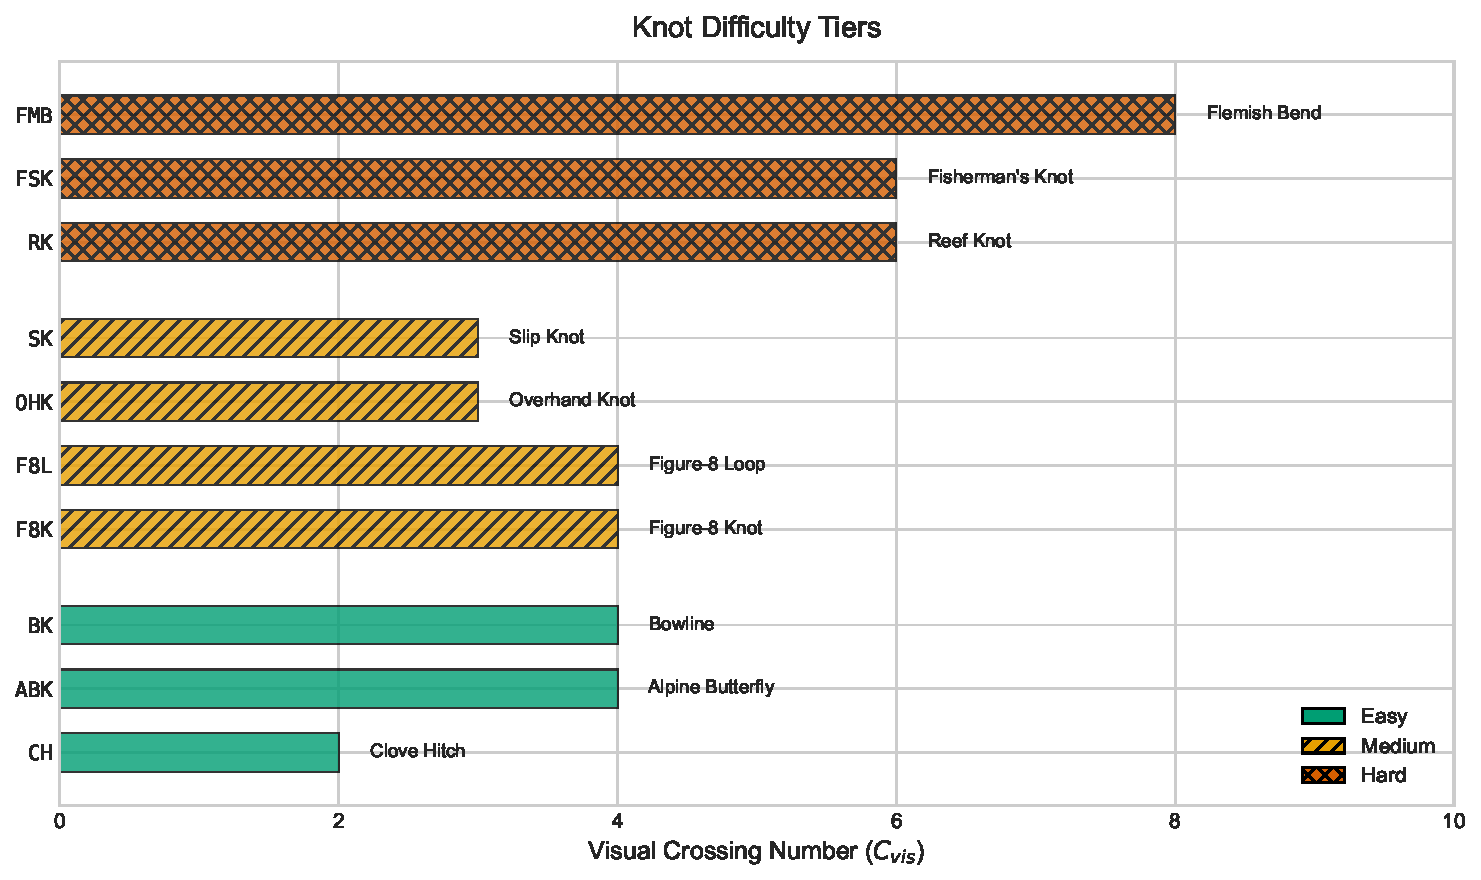
\includegraphics[width=0.9\linewidth]{difficulty_tiers.pdf}
\caption{Knot difficulty tiers based on topological properties. Bar length indicates visual crossing number.}
\label{fig:difficulty}
\end{figure}

\subsubsection{Weight Sensitivity}

To verify that our results are robust to the choice of distance metric weights (Section~\ref{sec:topo_metric}), we conducted a Monte Carlo sensitivity analysis. We perturbed each weight by up to $\pm 50\%$ and re-normalized to sum to 1.0, generating 200 random weight vectors. The resulting Spearman correlations (on EfficientNet-B0) have mean $\rho = -0.483 \pm 0.016$, with 100\% of perturbations yielding $\rho < -0.25$. Across all five general architectures, switching from the default to uniform weights ($w_f = 0.2$) changes $\rho$ by less than 0.01. Only extreme single-factor configurations (e.g., family membership alone) degrade the correlation to non-significance. These results indicate that the topological--visual correlation is a robust phenomenon, not an artifact of a particular weight choice (Supplementary Figure~\ref{fig:weight_sensitivity}).


% ============================================
% TOPOLOGICAL-VISUAL CORRELATION
% ============================================
\subsection{Topological-Visual Correlation Analysis}\label{sec:correlation}

We now validate the central hypothesis: that topological similarity predicts visual confusion. For each model, we extract the pairwise confusion rate $c(k_i, k_j)$ from the normalized confusion matrix and compute its correlation with the topological distance $d(k_i, k_j)$.

\subsubsection{Correlation Results}

Table~\ref{tab:correlation} reports Spearman and Pearson correlations between topological distance and pairwise confusion rate across all 45 knot pairs.

\begin{table}[t]
\centering
\caption{Correlation between topological distance and pairwise confusion rate, with Mantel permutation test significance. The Mantel $p$-value accounts for the non-independence of matrix entries via 9{,}999 random permutations \citep{mantel1967}.}
\label{tab:correlation}
\small
\begin{tabular}{@{}lcccc@{}}
\toprule
Model & Spearman $\rho$ & Pearson $r$ & Mantel $r$ & Mantel $p$ \\
\midrule
ResNet-18 & $-0.291$ & $-0.301$ & $-0.291$ & 0.058 \\
ResNet-50 & $-0.472$ & $-0.453$ & $-0.472$ & 0.002\rlap{$^{**}$} \\
EfficientNet-B0 & $-0.491$ & $-0.426$ & $-0.492$ & 0.001\rlap{$^{***}$} \\
ViT-B/16 & $-0.398$ & $-0.359$ & $-0.398$ & 0.005\rlap{$^{**}$} \\
Swin-T & $-0.214$ & $-0.195$ & $-0.214$ & 0.173 \\
\bottomrule
\multicolumn{5}{@{}l}{\footnotesize $^{**}p<0.01$; $^{***}p<0.001$. 9{,}999 permutations, two-tailed.}
\end{tabular}
\end{table}

Three of five general architectures show statistically significant negative correlations under the Mantel permutation test (negative correlation indicates that topologically similar knots are more frequently confused). The strongest association appears in EfficientNet-B0 (Mantel $r = -0.492$, $p = 0.001$), followed by ResNet-50 ($r = -0.472$, $p = 0.002$) and ViT-B/16 ($r = -0.398$, $p = 0.005$). ResNet-18 shows a marginally significant trend ($r = -0.291$, $p = 0.058$). The exception is Swin-T ($r = -0.214$, $p = 0.173$): as it produces extremely sparse confusion patterns (only 3 non-zero off-diagonal pairs out of 45), the correlation estimate becomes statistically underpowered.

\noindent\textbf{Mantel permutation test.} Since the 45 pairwise distances are derived from symmetric matrices and are not fully independent, standard parametric $p$-values may be liberal. We therefore apply the Mantel test \citep{mantel1967} with 9{,}999 random row--column permutations. The permutation-based $p$-values (Table~\ref{tab:correlation}) confirm that the negative correlation is significant at $p < 0.01$ for three models and marginally significant for a fourth, providing non-parametric evidence for the topological--visual association that accounts for the matrix structure of the data.

\subsubsection{Interpretation}

This result yields a clear interpretation: \emph{weaker models' errors are structured by knot theory, while stronger models produce too few errors for the correlation to reach significance}. The progression from ResNet-18 ($\rho = -0.291$) through EfficientNet-B0 ($\rho = -0.491$) to Swin-T ($\rho = -0.214$, n.s.) does not reflect a monotonic trend in correlation strength, but rather a transition from noisy errors (ResNet-18 makes enough errors but some are random) through topology-aligned errors (EfficientNet-B0 exhibits the strongest alignment between confusion structure and topological similarity) to near-elimination of errors (Swin-T).

The most confused pairs across models are consistent with topological predictions:
\begin{itemize}
    \item \textbf{F8K--OHK} ($d = 0.156$): Both derive from low-crossing prime knots ($4_1$ and $3_1$), sharing a single-loop stopper structure.
    \item \textbf{F8K--SK} ($d = 0.231$): SK is a slip variant of the trefoil, visually similar to F8K when tightly dressed.
    \item \textbf{FSK--FMB} ($d = 0.150$): Both are composite bend knots with intertwined rope segments.
\end{itemize}

Figure~\ref{fig:confusion} visualizes confusion matrices for the best-performing model (Swin-T) and a representative weaker model (ViT-B/16), illustrating how topological similarity manifests in systematic confusion patterns.

\begin{figure}[t]
\centering
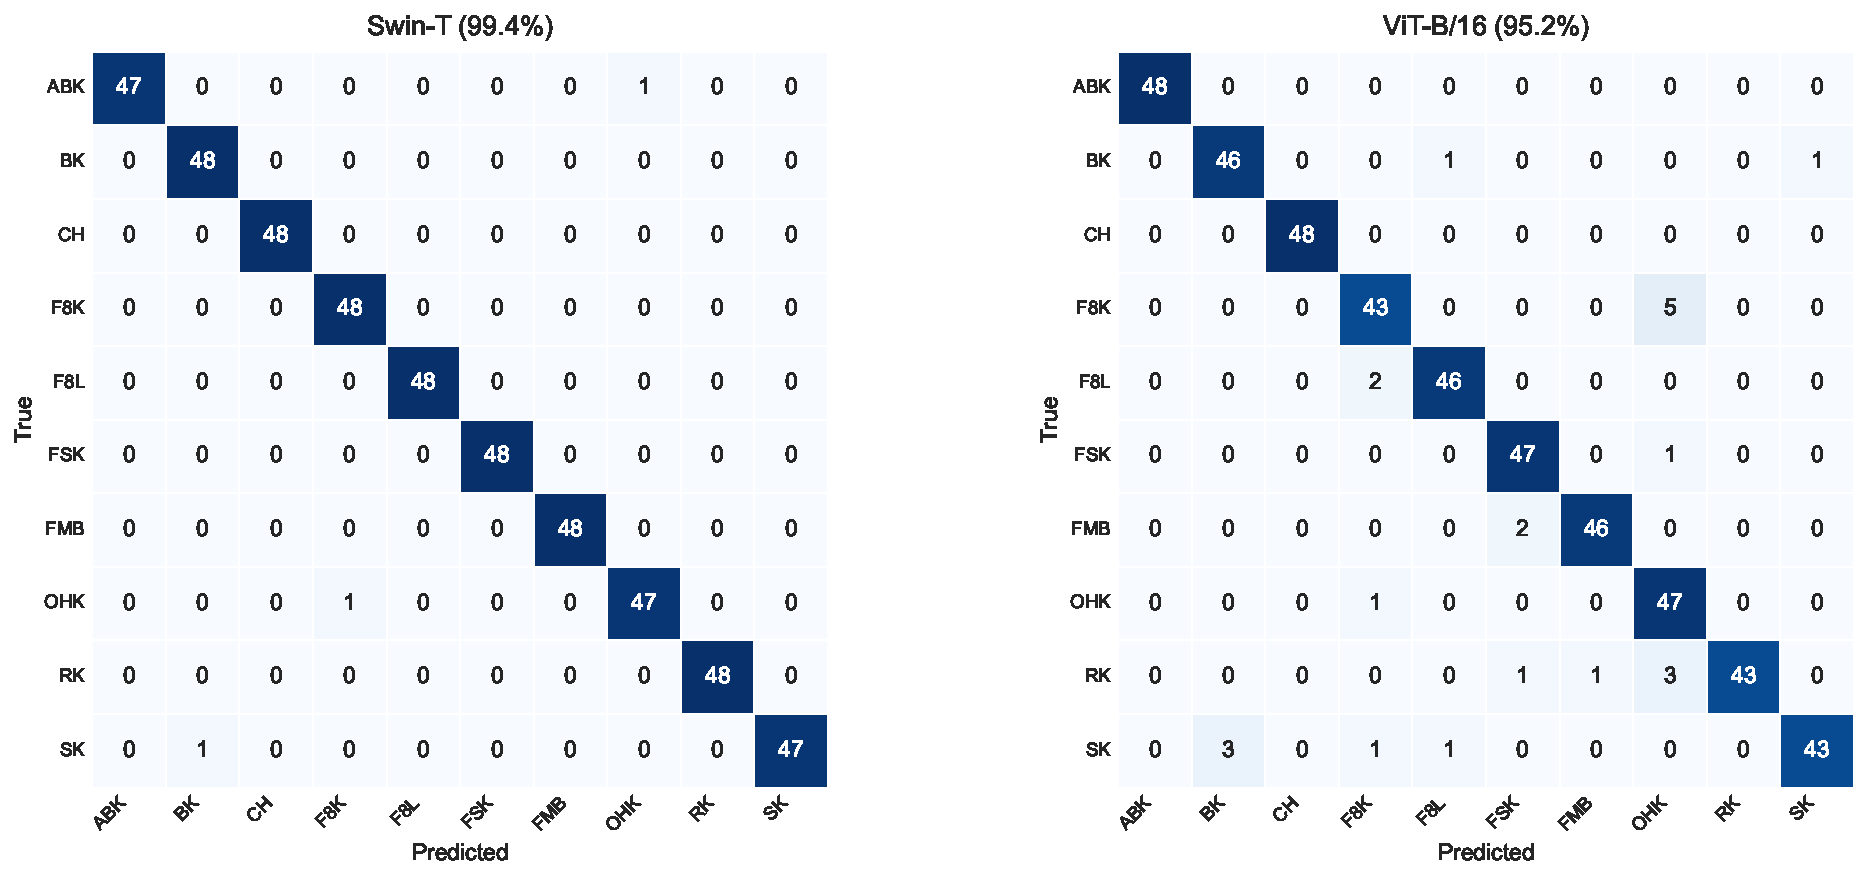
\includegraphics[width=\linewidth]{confusion_best_worst.pdf}
\caption{Confusion matrices for Swin-T (left) and ViT-B/16 (right). Rows are true labels, columns are predictions. Swin-T achieves near-perfect classification. ViT-B/16 shows systematic confusion between topologically similar knots: Figure-8 Knot vs.\ Overhand Knot (both prime stopper knots) and Fisherman's Knot vs.\ Flemish Bend (both composite bends). These patterns align with topological similarity (Section~\ref{sec:correlation}).}
\label{fig:confusion}
\end{figure}

\subsubsection{Grad-CAM Visualization}
\label{sec:gradcam}

To verify that models attend to knot-relevant image regions rather than background artifacts, we apply Gradient-weighted Class Activation Mapping (Grad-CAM) \citep{selvaraju2017gradcam} to ResNet-18 and ResNet-50. For our transformer-based models, attention-based interpretability methods \citep{chefer2021transformer} offer complementary insights. Supplementary Figure~\ref{fig:gradcam} shows activation heatmaps for one test image per class.

Both models consistently focus on the central knot structure, confirming that classification decisions are driven by rope crossing patterns rather than contextual cues such as the background surface. However, the two models differ in two respects:

\begin{itemize}
    \item \textbf{Spatial precision.} ResNet-50 produces tighter, more concentrated activation regions than ResNet-18, consistent with its deeper feature hierarchy enabling finer spatial discrimination.
    \item \textbf{Contextual leakage.} For Clove Hitch, ResNet-18's activation extends along the vertical pole, suggesting partial reliance on the mounting object rather than the knot topology itself. ResNet-50 shows less of this effect.
\end{itemize}


% ============================================
% TOPOLOGY-GUIDED REPRESENTATION LEARNING
% ============================================
\subsection{Topology-Guided Training Results}\label{sec:topo_results}

The correlation analysis in Section~\ref{sec:correlation} establishes that topological distance predicts visual confusion. This raises the question of whether such a topological prior can be exploited during training to produce more structured representations. We apply topology-guided training (see Section~\ref{sec:topo_method} for the method definition) and evaluate its impact on both classification accuracy and embedding quality.

\subsubsection{Classification Results}

We compare test accuracy between baseline (cross-entropy only) and topology-guided training (CE+TACA) on ResNet-18. Across three seeds (42, 123, 456), both configurations achieve comparable mean test accuracy ($96.88\%$ vs $96.81\%$), with similar cross-seed standard deviations ($1.06\%$ vs $1.00\%$; Supplementary Table~\ref{tab:robustness}). Under seed 42 specifically, TACA shows a 1.25-point gain ($95.83\% \to 97.08\%$), but McNemar paired tests confirm this is not statistically significant ($p = 0.48$; Table~\ref{tab:mcnemar}), with only 1--5 discordant pairs out of 480 test samples (standard error $\approx 0.9\%$). For ResNet-50 under seed 42, the difference is also negligible ($96.04\% \to 95.83\%$, $p = 1.00$). These results establish that \textbf{TACA does not improve mean classification accuracy or substantially reduce cross-seed variance}; its contribution lies in embedding restructuring, which we evaluate below.


\subsubsection{Loss Component Ablation}

A four-way ablation on ResNet-18 (Supplementary Table~\ref{tab:loss_ablation}) confirms that all loss configurations---CE only, CE+TACA, CE+TAML, and CE+TACA+TAML---achieve statistically indistinguishable mean accuracy ($96.0$--$96.9\%$). Combining both topology-guided losses introduces optimization instability (highest cross-seed variance: $1.47\%$). TACA's primary reproducible contribution is therefore embedding restructuring rather than classification-level improvements.

\subsubsection{Embedding Alignment Analysis}\label{sec:embedding_analysis}

Beyond classification accuracy, we hypothesize that topology-guided training restructures the learned feature space. To test this, we extract penultimate-layer embeddings from both baseline and topology-guided models, compute class centroid distance matrices, and measure their correlation with the topological distance matrix.

Table~\ref{tab:embed_align} reports Spearman and Pearson correlations between embedding centroid distances and topological distances across all 45 knot pairs.

\begin{table}[t]
\centering
\caption{Correlation between embedding centroid distances and topological distances. Topology-guided training significantly improves alignment: ResNet-18 increases from 0.462 to 0.645 (40\% improvement, $p < 0.001$); ResNet-50 from 0.495 to 0.641 (30\% improvement, $p < 0.001$).}
\label{tab:embed_align}
\small
\begin{tabular}{@{}lcccc@{}}
\toprule
Model & Spearman $\rho$ & $p$-value & Pearson $r$ & $p$-value \\
\midrule
ResNet-18 (baseline) & 0.462 & 0.001 & 0.480 & $<0.001$ \\
ResNet-18 (topo-guided) & \textbf{0.645} & $<0.001$ & \textbf{0.621} & $<0.001$ \\
\addlinespace
ResNet-50 (baseline) & 0.495 & $<0.001$ & 0.485 & $<0.001$ \\
ResNet-50 (topo-guided) & \textbf{0.641} & $<0.001$ & \textbf{0.608} & $<0.001$ \\
\bottomrule
\end{tabular}
\end{table}

For ResNet-18, the Spearman correlation increases by 40\% (from 0.462 to 0.645), while for ResNet-50 the increase is 30\% (from 0.495 to 0.641). All topology-guided correlations are significant at $p < 0.001$. Notably, the Mantel test on the topology-guided models' confusion matrices yields similar correlations to the baselines (ResNet-18: $r = -0.281$, $p = 0.065$; ResNet-50: $r = -0.453$, $p = 0.003$), indicating that TACA improves embedding geometry without substantially altering the confusion structure---consistent with its role as a representation regularizer rather than a classification loss.

\subsubsection{Visualization}

Supplementary Figure~\ref{fig:distance_comparison} compares the topological distance matrix with embedding centroid distance matrices from baseline and topology-guided ResNet-18. The baseline embedding distances show a relatively uniform pattern with limited contrast, while the topology-guided distances recover much of the structure present in the topological ground truth.


Figure~\ref{fig:tsne_umap} shows t-SNE \citep{vandermaaten2008tsne} and UMAP \citep{mcinnes2018umap} projections of the learned embeddings, colored by topological family. In the baseline embedding space, knots from the same family (e.g., the three loop knots: ABK, BK, F8L) are scattered across different regions. In the topology-guided space, same-family knots cluster together: loop knots group tightly, stopper knots are proximate, and bend knots occupy a shared region. Both dimensionality reduction methods yield consistent results, ruling out algorithm-specific artifacts.

\begin{figure}[t]
\centering
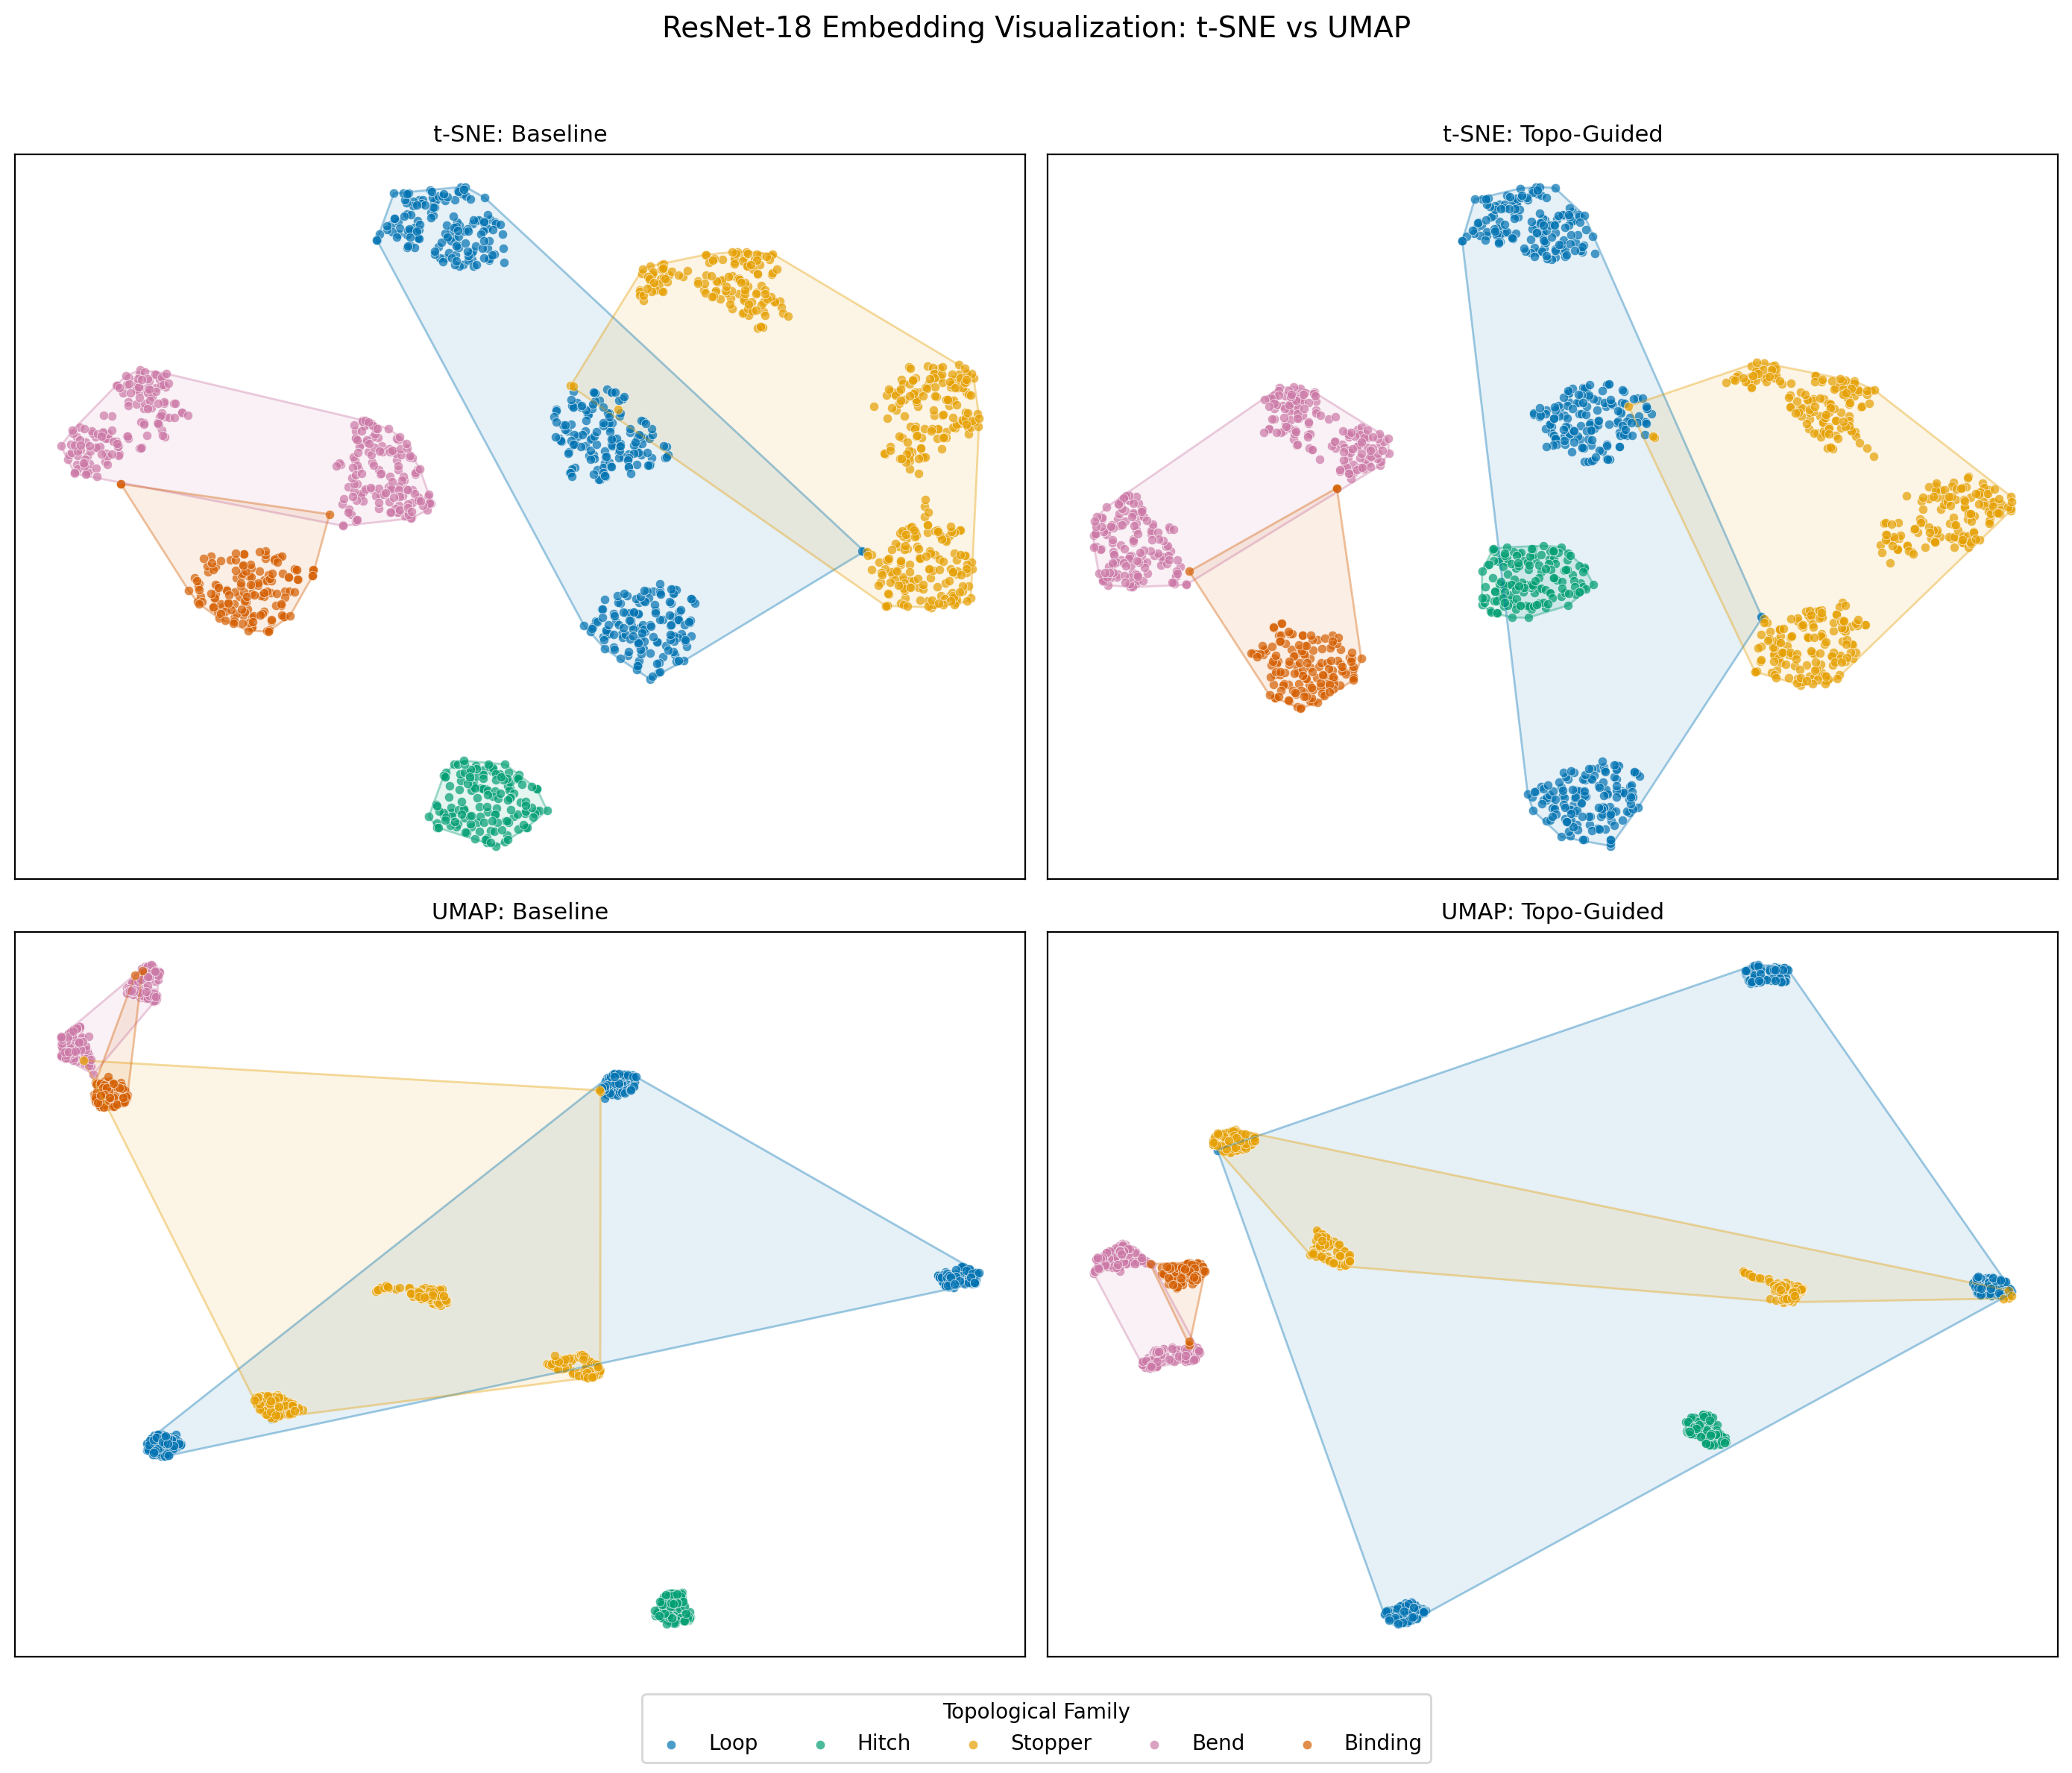
\includegraphics[width=\linewidth]{tsne_umap_comparison.png}
\caption{Comparison of t-SNE (top) and UMAP (bottom) projections of ResNet-18 embeddings. Left: baseline training; right: topology-guided training. Convex hulls indicate topological family boundaries. Both methods confirm that topology-guided training produces family-coherent clusters.}
\label{fig:tsne_umap}
\end{figure}

\subsubsection{Independent Validation: k-NN Retrieval}
\label{sec:knn}

A key concern with evaluating TACA via embedding--topology correlation is circularity: the training loss explicitly optimizes alignment, so measuring that alignment post hoc is partly tautological. To provide a genuinely independent assessment, we evaluate k-NN retrieval accuracy, which does not reference the topological distance matrix at evaluation time. For each test sample, we retrieve its $k$ nearest neighbors from the training set embeddings (cosine similarity) and predict the majority-vote label.

\begin{table}[t]
\centering
\caption{Independent validation of TACA's representation quality. k-NN retrieval accuracy (\%) uses cosine similarity; Mantel $\rho$ measures embedding--topology correlation ($n_\text{perm} = 9{,}999$). All results on seed 42, $n_\text{test} = 480$.}
\label{tab:independent_validation}
\small
\begin{tabular}{@{}lccccc@{}}
\toprule
Model & Method & k=1 & k=3 & k=5 & Mantel $\rho$ \\
\midrule
ResNet-18 & CE   & 96.88 & 96.04 & 96.25 & 0.468 \\
ResNet-18 & TACA & 96.67 & 96.25 & 95.83 & \textbf{0.618} \\
\addlinespace[2pt]
ResNet-50 & CE   & 95.83 & 95.63 & 95.83 & 0.514 \\
ResNet-50 & TACA & \textbf{97.08} & \textbf{97.08} & \textbf{97.08} & \textbf{0.727} \\
\bottomrule
\end{tabular}
\end{table}

For ResNet-18, k-NN accuracy is nearly identical between CE and TACA (within $\pm$0.4pp), consistent with the non-significant McNemar result. For ResNet-50, TACA improves k-NN by +1.25pp at all $k$ values, suggesting that the larger embedding space (2048-d) benefits more from topological structuring. Critically, k-NN retrieval does not use the topological distance matrix at evaluation time, yet TACA embeddings perform at least as well as CE embeddings---demonstrating that TACA's improvements reflect genuinely more discriminative features, not merely an artifact of the alignment loss.

\subsubsection{Random Distance Ablation}
\label{sec:random_ablation}

To determine whether TACA's benefits arise from the specific topological distance structure or from generic auxiliary-loss regularization, we train five ResNet-18 models: (1) CE only, (2) CE + real topological TACA, and (3--5) CE + TACA with randomly permuted distance matrices (seeds 1000--1002).

\begin{table}[t]
\centering
\caption{Random distance ablation on ResNet-18 (seed 42). Alignment $\rho$ measures Spearman correlation between embedding centroid distances and the \emph{real} topological distance matrix. Permuted TACA uses shuffled distance matrices during training but is evaluated against the real matrix. Note: absolute accuracy values differ from Table~\ref{tab:results} because the ablation models were trained in an independent run with different CUDA non-deterministic operations (see Supplementary Section~S8 for discussion); the relative comparisons within this table remain valid.}
\label{tab:ablation}
\small
\begin{tabular}{@{}lcccc@{}}
\toprule
Condition & Test Acc (\%) & k-NN ($k{=}1$, \%) & k-NN ($k{=}5$, \%) & Alignment $\rho$ \\
\midrule
CE only (no TACA) & 98.33 & 98.12 & 98.33 & 0.438 \\
Real TACA & 97.92 & 97.29 & 97.29 & \textbf{0.448} \\
\midrule
Permuted 1 (seed 1000) & 98.33 & 98.12 & 98.12 & 0.392 \\
Permuted 2 (seed 1001) & 97.92 & 97.50 & 97.50 & 0.425 \\
Permuted 3 (seed 1002) & 97.92 & 97.71 & 98.12 & 0.441 \\
\addlinespace[2pt]
\textit{Permuted mean} & \textit{98.06} & \textit{97.78} & \textit{97.92} & \textit{0.419} \\
\bottomrule
\end{tabular}
\end{table}

The results reveal a nuanced picture. All five conditions achieve indistinguishable accuracy (97.9--98.3\%) and k-NN retrieval, confirming that TACA does not improve classification regardless of the distance matrix used. Real TACA achieves the highest alignment $\rho$ (0.448) compared to the permuted mean (0.419, +7\%), but one permuted run (seed 1002, $\rho = 0.441$) nearly matches real TACA. \textbf{Most of TACA's regularization effect is therefore structure-agnostic}: adding any auxiliary centroid alignment loss---whether topologically structured or random---has a consistent regularization effect, with the specific topological structure contributing only a modest additional margin. This is an honest negative result that clarifies TACA's mechanism and the conditions under which topological priors add genuine value.

\subsubsection{Extensions}

To relax the assumption of hand-crafted distance weights, we extend TACA with learnable weight logits optimized end-to-end (Supplementary Section~S9, Supplementary Table~\ref{tab:learnable_weights}). Results are backbone-dependent: learnable-weight ResNet-50 achieves the best multi-seed mean ($96.53 \pm 0.43\%$), while ResNet-18 exhibits high seed sensitivity ($95.28 \pm 2.23\%$). Both backbones converge to similar weight distributions---upweighting structural derivation and type similarity---suggesting that the learned configuration reflects task structure. The embedding alignment ($\rho \approx 0.51$) is lower than hand-crafted TACA ($\rho \approx 0.64$), revealing an accuracy--alignment trade-off where the learnable weights optimize for classification rather than explicit distance alignment.

Preliminary cross-dataset experiments applying TACA to CUB-200-2011 \citep{wah2011cub} and FGVC-Aircraft \citep{maji2013fgvcaircraft} (Supplementary Section~S10) show that TACA fails when the domain distance metric does not reflect visual similarity, suggesting the Mantel test as a diagnostic tool before investing in representation-level regularization.


% ============================================
% 5. DISCUSSION
% ============================================
\section{Discussion}
\label{sec:discussion}

Our results counter the intuition that larger models necessarily yield better fine-grained performance. ViT-B/16, with three times the parameters of Swin-T, achieves lower accuracy, consistent with the known data-hunger of pure transformers \citep{dosovitskiy2021vit}. Swin-T's hierarchical shifted-window design appears well-suited to capturing both fine-grained rope crossing patterns and global knot topology. The 2.5--4\% validation-to-test accuracy gap across most architectures quantifies the domain shift from loose to tight knots, though ImageNet-pretrained features remain reasonably robust to this deformation.

The comparison with FGVC-specialized methods illuminates \emph{which} visual priors transfer to topological classification. Attention-based part selection succeeds by focusing on discriminative crossing regions, while graph-based spatial reasoning shows brittle seed sensitivity and jigsaw-based multi-granularity learning disrupts the continuous crossing topology that distinguishes knot types. No FGVC method significantly outperforms Swin-T, and multi-seed analysis reveals unstable method rankings (Supplementary Table~\ref{tab:robustness}), underscoring that single-seed comparisons can be misleading on small test sets.

With near-ceiling classification accuracy, the more informative question is whether topological structure explains classification difficulty. The Mantel permutation test provides a positive answer ($p < 0.01$ for three of five models), establishing that knot-theoretic distance predicts visual confusion patterns. We view this diagnostic capability as TACA's primary contribution: the Mantel test offers a computationally inexpensive, domain-agnostic method for determining \emph{whether} a candidate inter-class distance metric captures the structure of visual confusion \emph{before} committing to representation-level regularization. Our cross-dataset experiments (Supplementary Section~S10) validate this diagnostic role: TACA improves embedding alignment on Knots-10 (where the Mantel test is significant) but fails on CUB-200-2011 and FGVC-Aircraft (where the domain distance metrics do not predict confusion), confirming that the Mantel test reliably predicts when structure-guided training will be effective.

As a regularizer, TACA improves embedding--topology correlation by 40\% ($p < 0.001$), confirmed by independent k-NN retrieval validation (Table~\ref{tab:independent_validation}). However, TACA does not improve classification accuracy (CE and TACA produce comparable means: $96.9\%$ vs $96.8\%$), and the random-distance ablation (Table~\ref{tab:ablation}) reveals that permuted distance matrices produce comparable alignment values, indicating that the dominant mechanism is generic auxiliary-loss regularization rather than exploitation of knot-theoretic relationships. This finding clarifies the boundary: topological structure explains confusion patterns but does not, in its current formulation, improve classification. Future work should investigate whether richer distance metrics---perhaps learned from data---can widen the gap between structured and random regularization. Learnable distance weights show backbone-dependent behavior, with larger backbones providing more stable optimization (Supplementary Section~S9).

Synthesizing across experiments, three conclusions emerge. \emph{First}, Swin-T's near-ceiling accuracy establishes that further gains require new data or task reformulations rather than new architectures. \emph{Second}, model size and prior specificity are partially substitutable: capacity (Swin-T), attention-based selection (TransFG), and domain-specific priors (learnable-weight ResNet-50) achieve comparable performance, while the \emph{wrong} prior actively hurts (PMG). \emph{Third}, the Mantel permutation test emerges as a general-purpose diagnostic for FGVC: given any candidate inter-class distance metric, a significant Mantel correlation with the confusion matrix justifies investing in representation-level regularization, while a non-significant result redirects effort toward architecture or data improvements. Our cross-dataset experiments confirm this: TACA succeeds on Knots-10 (significant Mantel) and fails on CUB-200 and Aircraft (non-significant), validating the test's predictive utility.

A preliminary cross-domain evaluation with smartphone photographs exposes the most critical limitation of the current benchmark: under the seed-42 checkpoint, Swin-T drops from 99.4\% to 41.0\% and ResNet-18 from 95.8\% to 27.0\% when tested on images taken with a different rope, background, and camera (Table~\ref{tab:crossdomain_main}). Note that the in-domain values here are seed-42 single-run results; multi-seed means ($97.2 \pm 1.1\%$ and $96.9 \pm 1.1\%$, respectively; Table~\ref{tab:results}) confirm that the in-domain performance is representative.

\begin{table}[t]
\centering
\caption{Cross-domain evaluation on 100 smartphone photographs (seed-42 checkpoint, no fine-tuning). In-domain accuracy is the seed-42 test set result; see Table~\ref{tab:results} for multi-seed means.}
\label{tab:crossdomain_main}
\small
\begin{tabular}{@{}lcccc@{}}
\toprule
Model & In-Domain Acc & Cross-Domain Acc & Macro F1 & $\Delta$ Acc \\
\midrule
Swin-T   & 99.4\% & 41.0\% & 0.391 & $-58.4$ pp \\
ResNet-18 & 95.8\% & 27.0\% & 0.194 & $-68.8$ pp \\
\bottomrule
\end{tabular}
\end{table}

The controlled photography protocol (10 photographs per knot type, each varying one domain-shift factor; see Supplementary Section~S2 for the full protocol) enables attribution of accuracy changes to specific factors. Table~\ref{tab:crossdomain_factors} reports per-factor accuracy for Swin-T.

\begin{table}[t]
\centering
\caption{Per-factor accuracy breakdown for Swin-T on cross-domain photographs. Cond.\ ID refers to the photography protocol conditions (Table~\ref{tab:crossdomain_protocol}); $n$ is the number of images per condition (10 knot types $\times$ photos per condition). $\Delta$ indicates accuracy change relative to the baseline condition (rope color, material, and diameter all differ from training).}
\label{tab:crossdomain_factors}
\small
\begin{tabular}{@{}lcccc@{}}
\toprule
Domain-Shift Factor & Cond.\ ID & $n$ & Accuracy & $\Delta$ from Baseline \\
\midrule
Baseline (rope A, gray surface, indoor, overhead) & 1 & 10 & 40.0\% & --- \\
Viewing angle (45\textdegree/30\textdegree) & 2--3 & 20 & 40.0\% & $\pm 0.0$ pp \\
Looseness ($\pm$ angle) & 4--5 & 20 & 45.0\% & $+5.0$ pp \\
Background change (blue/beige surface) & 6--7 & 20 & 50.0\% & $+10.0$ pp \\
Natural lighting & 8 & 10 & 50.0\% & $+10.0$ pp \\
Rope material change (rope B) & 9 & 10 & 20.0\% & $-20.0$ pp \\
Combined shift (rope B + blue surface + natural) & 10 & 10 & 30.0\% & $-10.0$ pp \\
\bottomrule
\end{tabular}
\end{table}

Three findings emerge, though all per-factor estimates rest on only 10--20 images and should be interpreted as exploratory. (1) \textbf{Rope appearance is the dominant degradation factor.} Even the baseline condition---which simultaneously changes rope color (blue $\to$ white-red), material (synthetic $\to$ nylon), and diameter ($\sim$10~mm $\to$ $\sim$6~mm)---already reduces accuracy to 40\%. Because these three variables are confounded, we cannot attribute the drop to color alone. Switching to rope~B (black cotton, $\sim$4~mm) causes a further $-20$~pp drop; visual inspection reveals that the narrow, dark rope renders crossing structure nearly unresolvable even for human experts, suggesting that this drop reflects \emph{information loss} rather than mere domain shift. (2) \textbf{Background and lighting changes are surprisingly benign} ($+10$~pp or neutral), suggesting that ImageNet pretraining provides reasonable invariance to these variations. (3) \textbf{Clove Hitch retains 80\% recall}, consistent with the context shortcut identified by Grad-CAM (Section~\ref{sec:gradcam}): the distinctive cross-shaped layout is preserved across domains, even though the rope itself changes. This is consistent with known texture bias in CNNs \citep{geirhos2019imagenettrained}: models encode rope appearance as a discriminative shortcut rather than relying on crossing topology alone. This 58--69~pp accuracy gap quantifies the distance between controlled benchmark performance and practical deployment, and motivates future work on color-invariant training, multi-material data collection, and domain adaptation.

We note four limitations. First, the single rope type limits generalization, as quantified by the cross-domain evaluation above. Second, the topological distance metric is a heuristic with manually selected factors; a fully data-driven metric remains future work. Third, the 480-sample test set limits statistical power: accuracy differences below $\sim$2 pp are not distinguishable, and multi-seed analysis confirms method ranking instability within this range. Fourth, topology-guided training was evaluated only on ResNet-18 and ResNet-50; its effect on Swin-T was not tested due to the near-perfect baseline.


% ============================================
% 6. CONCLUSION
% ============================================
\section{Conclusion}
\label{sec:conclusion}

In summary, we have presented Knots-10, a tightness-stratified benchmark for physical knot classification. Among eight architectures, Swin-T achieves the highest accuracy through model capacity, while FGVC-specialized methods show mixed results: TransFG succeeds through attention-based part selection, while PMG's jigsaw strategy is counterproductive. Our central analytical contribution is the topological difficulty framework: the Mantel permutation test reveals a statistically significant link between knot-theoretic similarity and visual confusion ($p < 0.01$ for three of five models), and TACA demonstrates that this structure can organize learned representations, though it does not translate into accuracy gains. Cross-dataset experiments (Supplementary Section~S10) suggest the Mantel test as a general diagnostic for when representation-level regularization may be warranted.

Future work will extend the dataset to additional knot types and rope materials to evaluate cross-material generalization, investigate data-driven distance metrics, and explore whether topology-aware representations improve few-shot generalization to novel knot types.


% ============================================
% END MATTER
% ============================================

\section*{Declaration of Competing Interest}

The authors declare that they have no known competing financial interests or personal relationships that could have appeared to influence the work reported in this paper.

\section*{CRediT Authorship Contribution Statement}

\textbf{Shiheng Nie}: Methodology, Software, Validation, Formal analysis, Investigation, Data curation, Writing -- original draft, Visualization. \textbf{Yunguang Yue}: Conceptualization, Supervision, Writing -- review \& editing.

\section*{Declaration of Generative AI and AI-Assisted Technologies in the Writing Process}

During the preparation of this work the authors used Gemini (Google) to assist with language polishing. After using this tool, the authors reviewed and edited the content as needed and take full responsibility for the content of the published article.

\section*{Data and Code Availability}

The 10Knots dataset is publicly available at \url{https://www.kaggle.com/datasets/josephcameron/10knots} under a CC BY-SA 4.0 license. Our evaluation code, trained model checkpoints, and analysis scripts are publicly available at \url{https://github.com/Mousaee/knots10-benchmark}.

\section*{Acknowledgements}

This work was inspired by the graduate course \emph{Deep Intelligent Computing and Practice} at Shihezi University. This research received no specific grant from any funding agency in the public, commercial, or not-for-profit sectors.

\bibliographystyle{elsarticle-num}
\bibliography{references}

\clearpage
\appendix
\renewcommand{\thefigure}{S\arabic{figure}}
\renewcommand{\thetable}{S\arabic{table}}
\renewcommand{\theHfigure}{S\arabic{figure}}
\renewcommand{\theHtable}{S\arabic{table}}
\setcounter{figure}{0}
\setcounter{table}{0}

\section*{Appendix A. Supplementary Material}\label{sec:appendix}

\subsection*{S1. Multi-Seed Robustness Analysis}\label{sec:supp_robustness}

All main-paper results report the mean $\pm$ standard deviation across three random seeds (42, 123, 456). Each configuration was trained from scratch under identical hyperparameters, with only the random seed affecting weight initialization, data shuffling, and the train/validation split. Table~\ref{tab:robustness} reports the per-configuration breakdown of test accuracy and macro F1 across the three runs.

\begin{table}[htbp]
\centering
\caption{Multi-seed robustness analysis. Each configuration is trained with three random seeds (42, 123, 456) and evaluated on the tightness-stratified test set. All other hyperparameters are held constant.}
\label{tab:robustness}
\small
\begin{tabular}{@{}lcc@{}}
\toprule
Configuration & Test Accuracy (\%) & Macro F1 \\
\midrule
ResNet-18 (CE)             & $96.88 \pm 1.06$ & $0.969 \pm 0.011$ \\
ResNet-18 (CE + TACA)      & $96.81 \pm 1.00$ & $0.968 \pm 0.010$ \\
ResNet-18 (CE + TAML)      & $96.53 \pm 0.79$ & $0.965 \pm 0.008$ \\
ResNet-18 (CE + TACA + TAML) & $95.97 \pm 1.47$ & $0.960 \pm 0.014$ \\
\midrule
ResNet-50 (CE)             & $95.83 \pm 1.03$ & $0.959 \pm 0.010$ \\
EfficientNet-B0 (CE)       & $96.25 \pm 0.45$ & $0.963 \pm 0.005$ \\
ViT-B/16 (CE)              & $96.39 \pm 0.35$ & $0.964 \pm 0.003$ \\
\textbf{Swin-T (CE)}       & $\mathbf{97.22 \pm 1.09}$ & $\mathbf{0.972 \pm 0.011}$ \\
\midrule
\multicolumn{3}{@{}l}{\textit{FGVC-Specialized Methods}} \\
\addlinespace[2pt]
TransFG (CE)               & $97.15 \pm 0.94$ & $0.972 \pm 0.010$ \\
PMG (CE)                   & $94.51 \pm 1.75$ & $0.945 \pm 0.018$ \\
Graph-FGVC (CE)            & $95.49 \pm 2.84$ & $0.955 \pm 0.028$ \\
\midrule
\multicolumn{3}{@{}l}{\textit{Topology-Guided Variants}} \\
\addlinespace[2pt]
ResNet-18 (CE + TACA learnable) & $95.28 \pm 2.23$ & $0.953 \pm 0.022$ \\
ResNet-50 (CE + TACA learnable) & $96.53 \pm 0.43$ & $0.966 \pm 0.004$ \\
\bottomrule
\end{tabular}
\end{table}

Table~\ref{tab:loss_ablation} presents the loss component ablation on ResNet-18, comparing CE only, CE+TACA, CE+TAML, and the combined CE+TACA+TAML configuration.

\begin{table}[htbp]
\centering
\caption{Ablation study of loss components on ResNet-18 (mean $\pm$ std across seeds 42, 123, 456). All configurations achieve comparable mean accuracy. TAML alone yields the lowest cross-seed variance (std: $0.79\%$), while the combined configuration (CE+TACA+TAML) shows the highest variance ($1.47\%$).}
\label{tab:loss_ablation}
\small
\begin{tabular}{@{}lcc@{}}
\toprule
Loss Configuration & Test Acc (\%) & Macro F1 \\
\midrule
CE only & $96.88 \pm 1.06$ & $0.969 \pm 0.011$ \\
CE + TACA & $96.81 \pm 1.00$ & $0.968 \pm 0.010$ \\
CE + TAML & $96.53 \pm \mathbf{0.79}$ & $0.965 \pm 0.008$ \\
CE + TACA + TAML & $95.97 \pm 1.47$ & $0.960 \pm 0.014$ \\
\bottomrule
\end{tabular}
\end{table}

The multi-seed data support four conclusions: (1)~Most configurations are stable (std $< 1.5\%$), with Graph-FGVC (2.84\%), learnable-weight ResNet-18 (2.23\%), and PMG (1.75\%) as exceptions. (2)~The general-architecture ranking Swin-T $>$ ResNet-18 $\approx$ ViT-B/16 $\approx$ EfficientNet-B0 $>$ ResNet-50 holds in aggregate. (3)~FGVC method ranking is highly unstable across seeds: the ranking changes under every seed, underscoring that single-seed comparisons among methods with overlapping confidence intervals can be misleading. (4)~Learnable weight optimization is backbone-dependent: ResNet-18 exhibits the highest variance ($95.28 \pm 2.23\%$), while ResNet-50 achieves the most stable result of any topology-guided configuration ($96.53 \pm 0.43\%$).

\emph{Note on Swin-T reproducibility:} The Swin-T seed-42 result in Table~\ref{tab:robustness} (98.75\%) differs from Table~\ref{tab:results} (99.38\%) due to non-deterministic CUDA operations in shifted-window attention. The multi-seed statistics in Table~\ref{tab:robustness} are computed from the robustness experiment's own runs to ensure internal consistency.

\subsection*{S2. Cross-Domain Evaluation with Phone Photographs}\label{sec:supp_crossdomain}

To provide a preliminary assessment of cross-domain generalization, we collected 100 photographs (10 knot types $\times$ 10 images) using a smartphone camera under non-laboratory conditions. No calibration or illumination standardization was applied beyond the protocol described below; this deliberately mimics a practical deployment scenario. The training set uses blue synthetic climbing rope on a dark background under controlled studio lighting; cross-domain images use two alternative ropes (white-red braided nylon cord and black braided cotton cord), three different backgrounds (light gray surface, blue surface, and beige surface), two lighting conditions (indoor artificial and natural window light), and multiple viewing angles (overhead, 45\textdegree, and 30\textdegree). The domain shift thus simultaneously involves changes in rope color (blue $\to$ white-red or black), rope material (synthetic climbing rope $\to$ braided nylon or cotton), rope diameter ($\sim$10~mm $\to$ $\sim$6~mm or $\sim$4~mm), and background appearance---these factors are partially confounded and cannot be fully isolated. For knot types that require two rope strands (Clove Hitch, Reef Knot, Fisherman's Knot, Flemish Bend), a second gray braided nylon cord was used as the paired strand. Each photograph systematically varies one or more domain-shift factors relative to a baseline condition (Table~\ref{tab:crossdomain_protocol}).

\begin{table}[htbp]
\centering
\caption{Cross-domain photography protocol. Each of the 10 photographs per knot type varies specific domain-shift factors relative to the training distribution. Photo 1 serves as the baseline (closest to training conditions except for rope color/material).}
\label{tab:crossdomain_protocol}
\small
\resizebox{\linewidth}{!}{%
\begin{tabular}{@{}clcccc@{}}
\toprule
Photo & Factor Tested & Tightness & Angle & Background & Rope \\
\midrule
1 & Baseline & Tight & 90\textdegree & Gray & A \\
2--3 & Viewing angle & Tight & 45\textdegree/30\textdegree & Gray & A \\
4--5 & Looseness ($\pm$ angle) & Loose & 90\textdegree/45\textdegree & Gray & A \\
6--7 & Background & Tight & 90\textdegree & Blue/Beige & A \\
8 & Lighting & Tight & 90\textdegree & Gray & A$^{\dagger}$ \\
9 & Rope material & Tight & 90\textdegree & Gray & B \\
10 & Combined shift & Tight & 90\textdegree & Blue & B$^{\dagger}$ \\
\bottomrule
\end{tabular}%
}
\vspace{0.3em}

\raggedright\footnotesize $^{\dagger}$Natural light; all other photos use indoor artificial light. Rope A: white-red braided nylon cord ($\sim$6~mm); Rope B: black braided cotton cord ($\sim$4~mm). Both differ substantially from the training rope (blue synthetic climbing rope, $\sim$10~mm) in color, material, and diameter.
\end{table}

\subsubsection*{Overall Results and Per-Factor Analysis}

Overall cross-domain performance and per-factor accuracy breakdown are presented in the main text (Tables~\ref{tab:crossdomain_main} and~\ref{tab:crossdomain_factors}, Section~\ref{sec:discussion}).

\subsubsection*{Per-Class Analysis}

Per-class accuracy reveals that certain knot types are more robust to domain shift than others. For Swin-T, Overhand Knot (OHK) achieves 90\% cross-domain recall, likely due to its simple and distinctive visual structure. Clove Hitch (CH) maintains 80\% recall, consistent with its unique two-loop-around-pole appearance. In contrast, Bowline (BK) and Flemish Bend (FMB) drop to 0\%, suggesting these knots' diagnostic visual features are heavily dependent on the specific rope appearance in the training data.

\subsubsection*{Interpretation}

The severe accuracy degradation is dominated by rope appearance. Critically, the baseline condition (Photo~1) already changes three variables simultaneously relative to the training distribution: rope color (blue $\to$ white-red), material (synthetic climbing rope $\to$ braided nylon), and diameter ($\sim$10~mm $\to$ $\sim$6~mm). Because these factors are confounded, the 40\% baseline accuracy cannot be attributed to color alone. Switching to rope~B (black braided cotton, $\sim$4~mm) causes an additional $-20$~pp drop; visual inspection of the rope~B photographs reveals that crossing structure---the primary discriminative feature for knot classification---becomes nearly unresolvable at this diameter and color combination, particularly for compact knots such as OHK and F8K. This suggests that the rope~B accuracy drop reflects genuine \emph{information loss} (the signal is physically absent from the image) rather than mere distributional shift that a more robust model could overcome. Background and lighting changes are surprisingly benign ($+10$~pp or neutral), suggesting reasonable invariance from ImageNet pretraining. Despite both models degrading substantially, Swin-T (41.0\%) maintains a 14-point advantage over ResNet-18 (27.0\%). The high cross-domain recall for Clove Hitch (80\% for Swin-T) is consistent with the context shortcut identified by Grad-CAM in the in-domain analysis (Section~\ref{sec:gradcam}): the distinctive cross-shaped layout (rope wrapped around a post) is preserved even when the rope appearance changes, confirming that models partly rely on scene geometry rather than crossing topology for this class.

\noindent\textbf{Caveat.} This evaluation was conducted by a single photographer using consumer smartphones under non-laboratory conditions, with no calibration or standardization beyond the protocol in Table~\ref{tab:crossdomain_protocol}. The sample size is small (100 images, 10 per class), and per-factor accuracy estimates are each based on only 10--20 images, making differences below $\sim$20~pp statistically unreliable. This deliberately mimics a realistic deployment scenario but limits the statistical rigor of per-factor attribution. A rigorous cross-domain benchmark would require multiple photographers, independent control of rope color/material/diameter, and substantially larger sample sizes.

\subsection*{S3. Supplementary Figures}\label{sec:supp_figures}

The following figures are referenced in the main text and provide supporting detail for the analyses presented therein.

\begin{figure}[htbp]
\centering
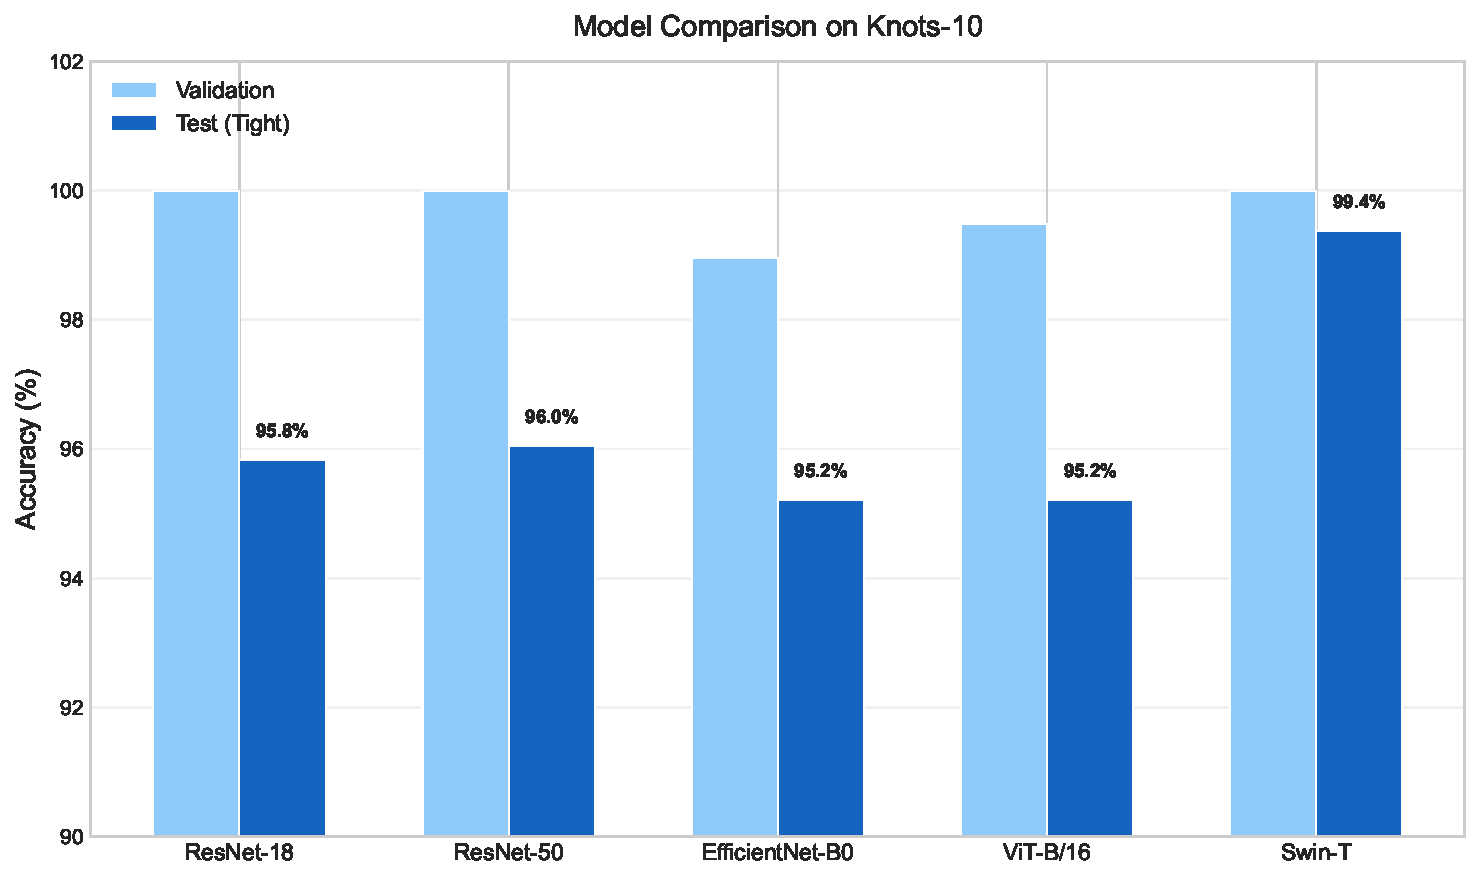
\includegraphics[width=\linewidth]{model_comparison.pdf}
\caption{Validation and test accuracy across all eight architectures (five general-purpose, three FGVC-specialized), seed 42 (CUDA rerun). Models are grouped by category with a visual separator. Swin-T achieves the highest test accuracy (98.8\%), followed by ViT-B/16 (96.9\%) and TransFG (96.3\%). Graph-FGVC (94.2\%) underperforms under this seed, though it reaches 98.8\% under seed 456. See Supplementary Table~\ref{tab:robustness} for multi-seed results.}
\label{fig:comparison}
\end{figure}

\begin{figure}[htbp]
\centering
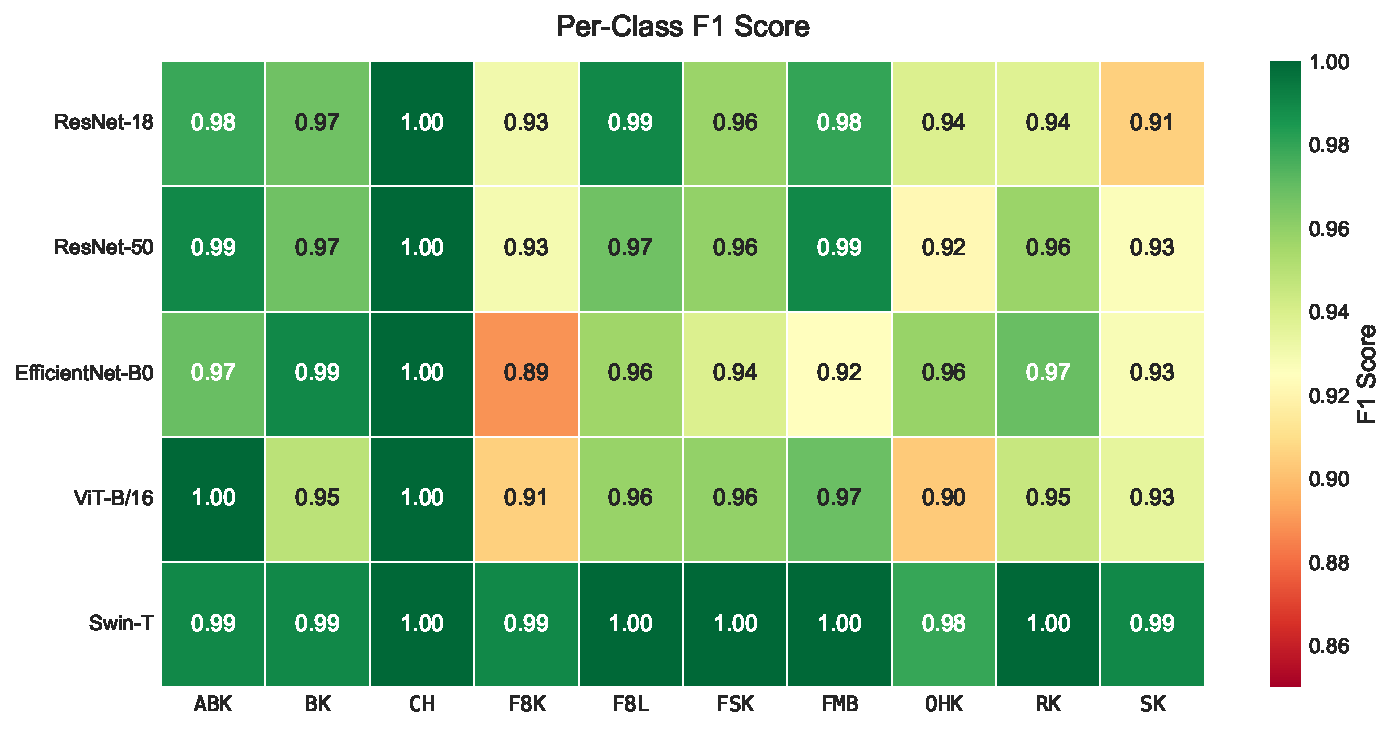
\includegraphics[width=\linewidth]{f1_heatmap.pdf}
\caption{Per-class F1 scores across all eight architectures (five general-purpose, three FGVC-specialized), seed 42 (CUDA rerun). Darker green indicates higher F1. A horizontal line separates General and FGVC-Specialized models. Clove Hitch (CH) achieves perfect scores across all models, while Figure-8 Knot (F8K) is consistently the most challenging class (F1 as low as 0.81 for ViT-B/16). Graph-FGVC shows notably lower F1 for OHK (0.86) and F8K (0.86), reflecting its seed sensitivity under this initialization.}
\label{fig:f1heatmap}
\end{figure}

\begin{figure}[htbp]
\centering
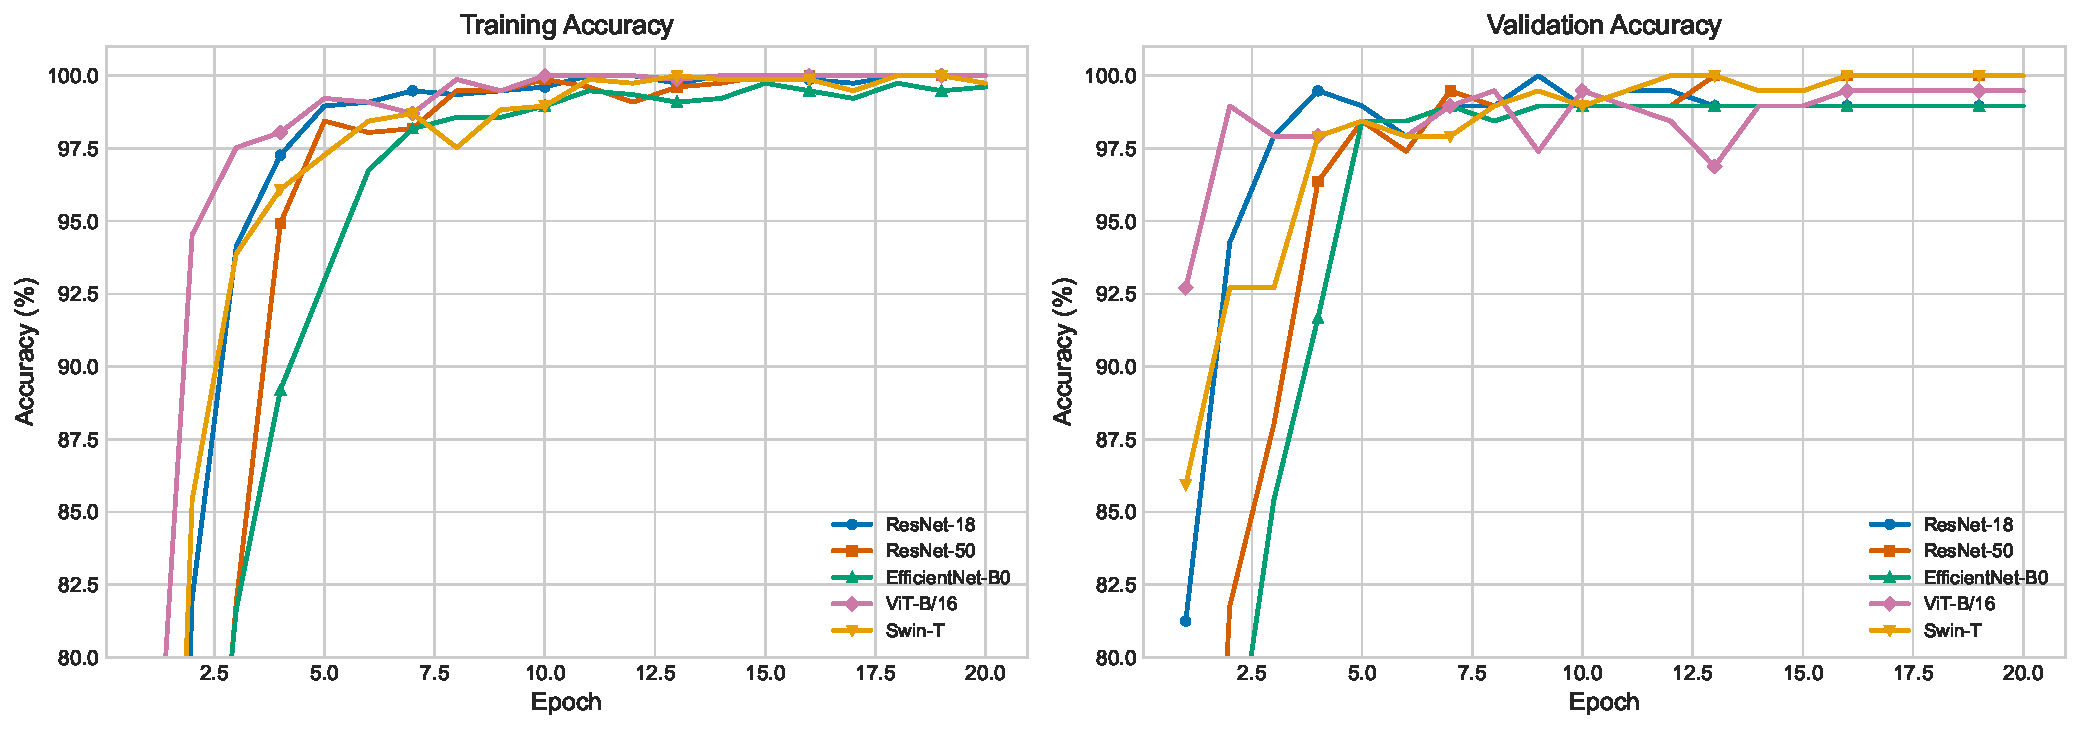
\includegraphics[width=\linewidth]{convergence_all.pdf}
\caption{Training and validation accuracy curves for all eight architectures over 20 epochs, organized in a 2$\times$2 grid. Top row: five general-purpose architectures (all converge within 10 epochs). Bottom row: three FGVC-specialized methods. PMG exhibits notably slower convergence due to its progressive multi-granularity training strategy.}
\label{fig:convergence}
\end{figure}

\begin{figure}[htbp]
\centering
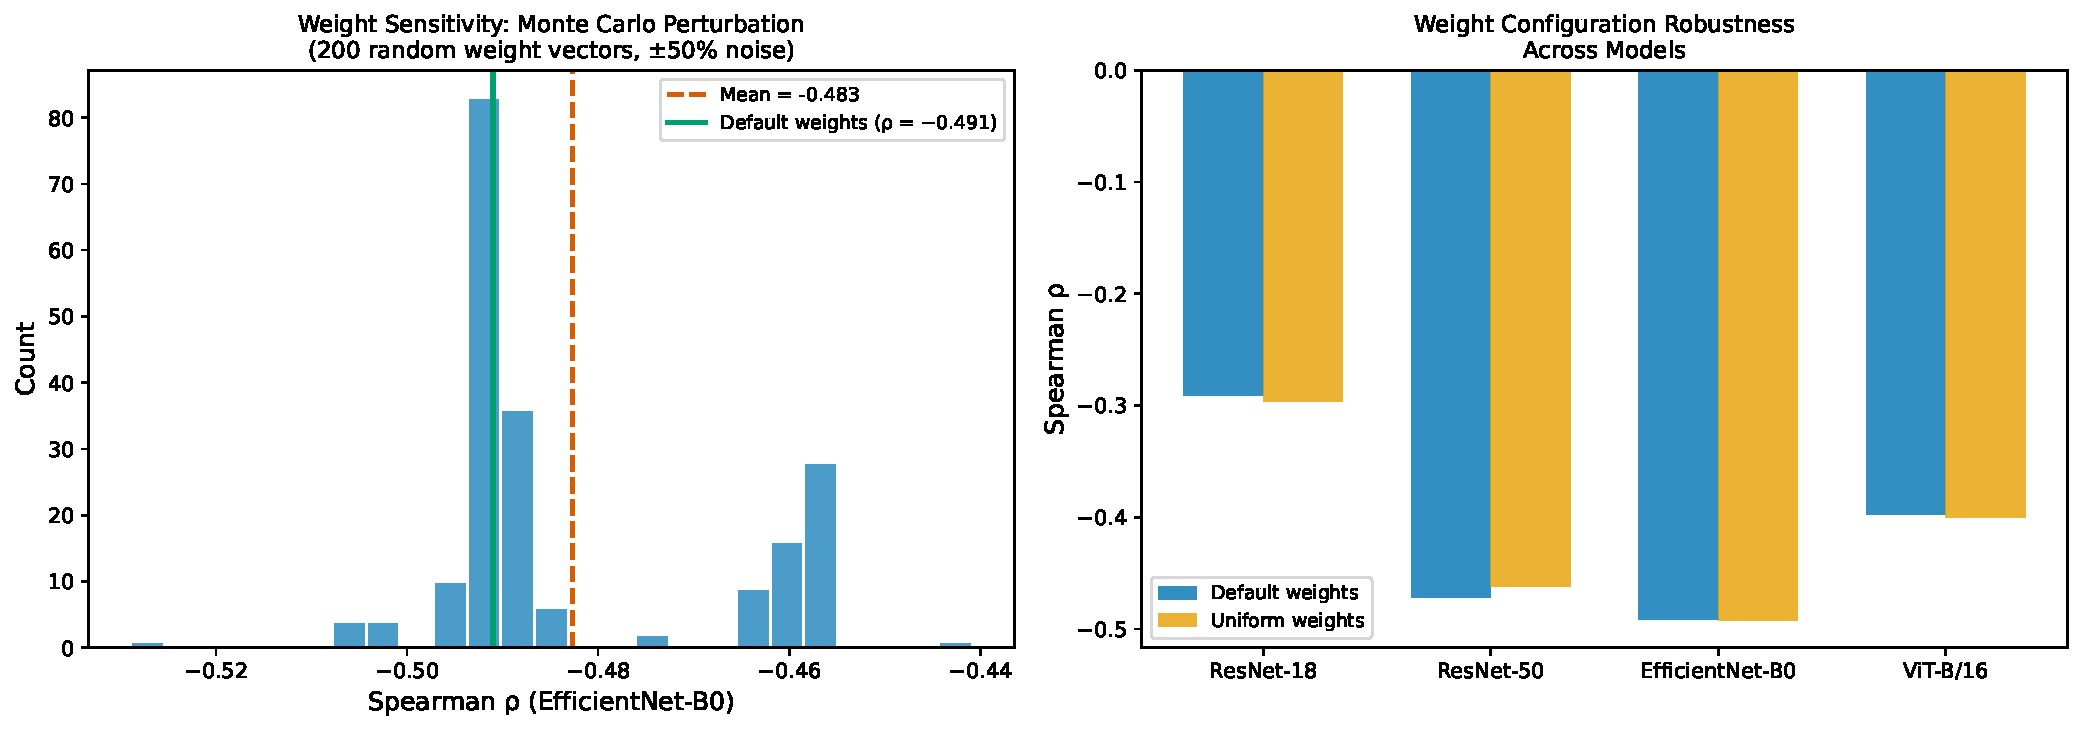
\includegraphics[width=\linewidth]{weight_sensitivity.pdf}
\caption{Weight sensitivity analysis. Left: distribution of Spearman $\rho$ across 200 random weight perturbations ($\pm 50\%$) for EfficientNet-B0. The correlation remains consistently negative ($\rho = -0.483 \pm 0.016$). Right: comparison of default and uniform weight configurations across all five general architectures, showing negligible differences.}
\label{fig:weight_sensitivity}
\end{figure}

\begin{figure}[htbp]
\centering
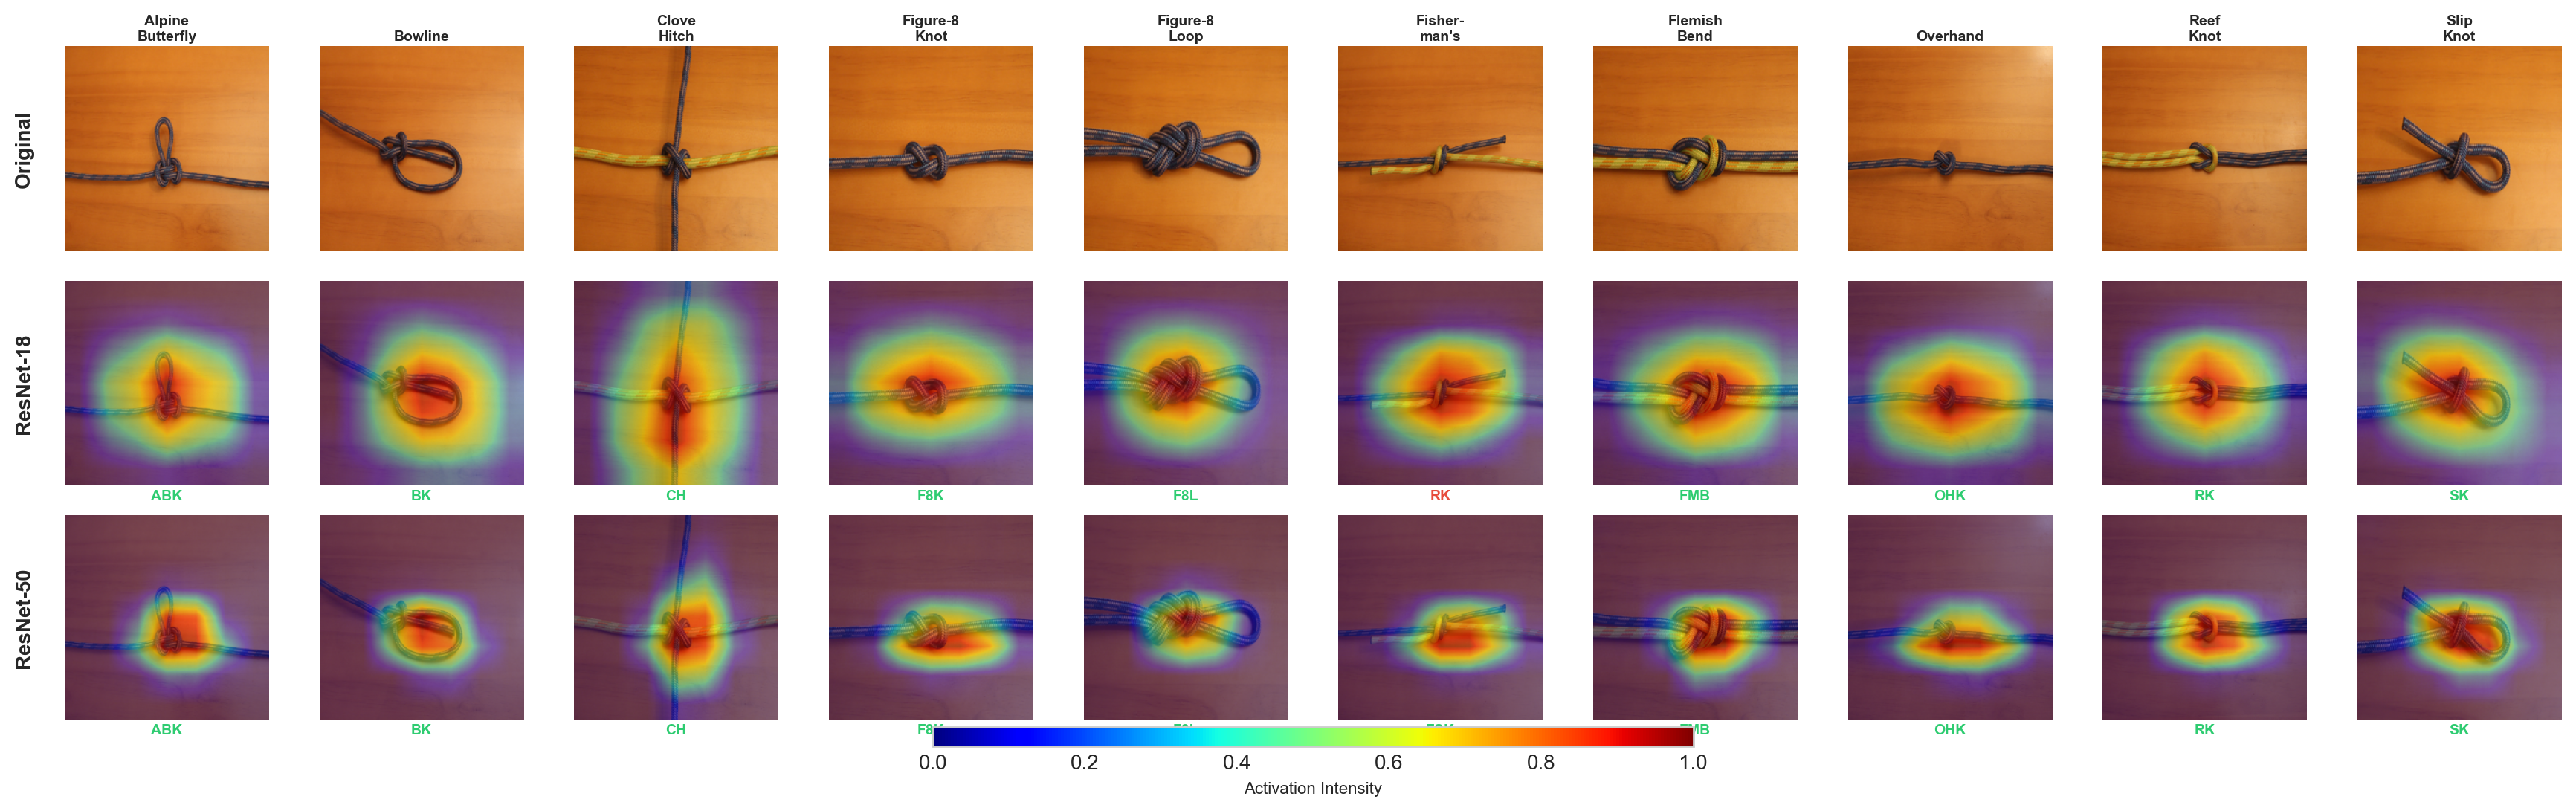
\includegraphics[width=\linewidth]{gradcam_comparison.pdf}
\caption{Grad-CAM visualizations for ResNet-18 (middle row) and ResNet-50 (bottom row) across all 10 knot classes. Top row shows original test images. Heatmaps overlay activation intensity (red = high, blue = low). Green labels indicate correct predictions, red labels indicate errors. Both models focus on the central knot structure. ResNet-50 produces more spatially concentrated activations than ResNet-18.}
\label{fig:gradcam}
\end{figure}

\begin{figure}[htbp]
\centering
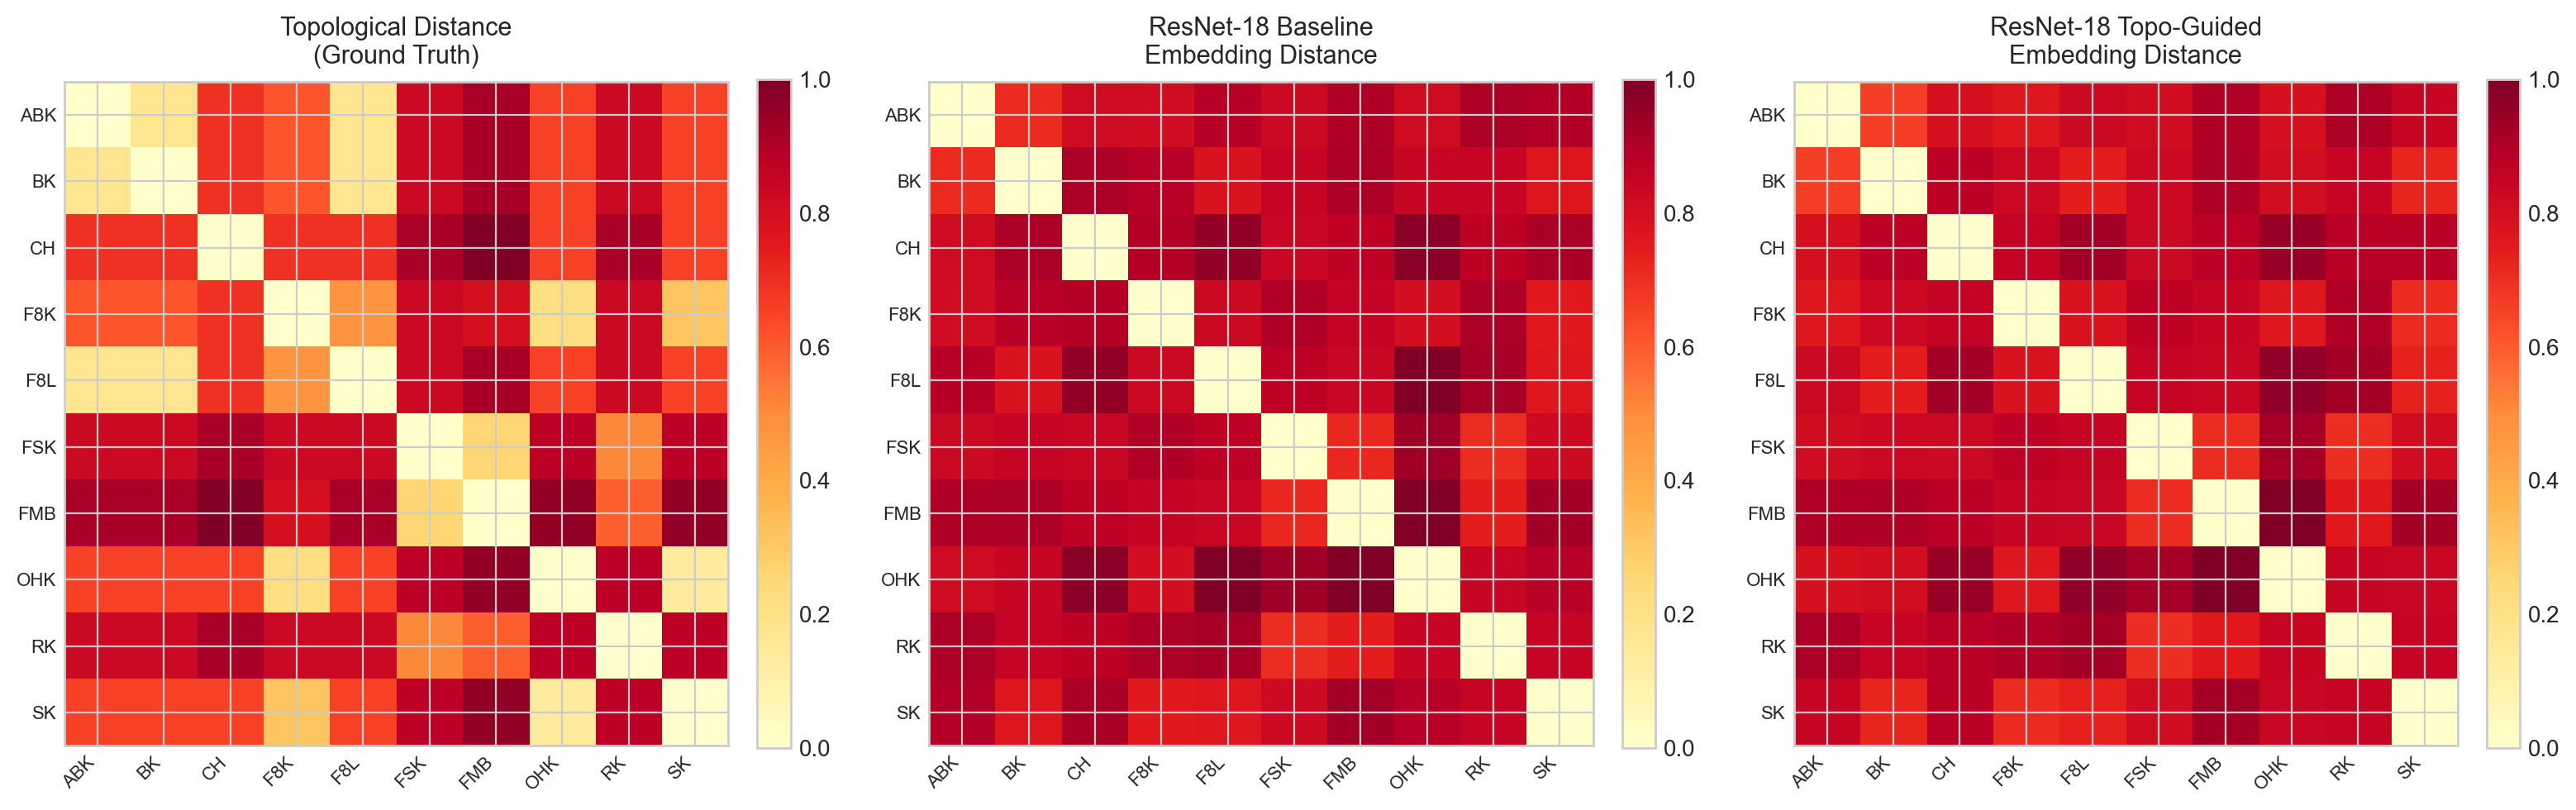
\includegraphics[width=\linewidth]{distance_comparison_resnet18.png}
\caption{Distance matrix comparison for ResNet-18. Left: topological distance (ground truth). Center: baseline embedding distances. Right: topology-guided embedding distances. Color intensity represents distance magnitude (darker = larger). The topology-guided embedding recovers topological structure with block patterns indicating family-level clustering.}
\label{fig:distance_comparison}
\end{figure}

\begin{table}[htbp]
\centering
\caption{Complete $\delta_5$ (structural derivation) matrix for all 45 knot pairs. Four pairs with known shared mathematical structure receive reduced penalties; all other pairs default to 0.5. Together with Table~\ref{tab:knot_taxonomy}, this table enables full reproduction of the $10 \times 10$ topological distance matrix.}
\label{tab:delta5}
\small
\resizebox{\linewidth}{!}{%
\begin{tabular}{@{}lcccccccccc@{}}
\toprule
 & OHK & SK & F8K & BK & F8L & ABK & CH & RK & FSK & FMB \\
\midrule
OHK & --- & 0.10 & 0.50 & 0.50 & 0.50 & 0.50 & 0.50 & 0.50 & 0.50 & 0.50 \\
SK  &     & --- & 0.50 & 0.50 & 0.50 & 0.50 & 0.50 & 0.50 & 0.50 & 0.50 \\
F8K &     &     & --- & 0.50 & 0.10 & 0.50 & 0.50 & 0.50 & 0.50 & 0.15 \\
BK  &     &     &     & --- & 0.50 & 0.50 & 0.50 & 0.50 & 0.50 & 0.50 \\
F8L &     &     &     &     & --- & 0.50 & 0.50 & 0.50 & 0.50 & 0.50 \\
ABK &     &     &     &     &     & --- & 0.50 & 0.50 & 0.50 & 0.50 \\
CH  &     &     &     &     &     &     & --- & 0.50 & 0.50 & 0.50 \\
RK  &     &     &     &     &     &     &     & --- & 0.10 & 0.50 \\
FSK &     &     &     &     &     &     &     &     & --- & 0.50 \\
FMB &     &     &     &     &     &     &     &     &     & --- \\
\bottomrule
\end{tabular}%
}
\end{table}

\subsection*{S4. Learnable Weight Evolution}\label{sec:supp_weights}

Figure~\ref{fig:weight_evolution} shows how the five learnable distance weights evolve across training epochs for ResNet-18. All weights are initialized at the uniform value $w_f = 0.2$ (corresponding to logits $\ell_f = 0$). During training, the weights diverge from uniformity and converge to a stable configuration by approximately epoch 10.

The final learned weight distribution $\mathbf{w}^*_{18} = (0.157, 0.225, 0.229, 0.153, 0.237)$ reveals interpretable structure: the model upweights structural derivation ($w_5$, from 0.20 to 0.24) and type similarity ($w_3$, from 0.20 to 0.23), while downweighting crossing number ($w_1$, from 0.20 to 0.16) and component count ($w_4$, from 0.20 to 0.15). This pattern is consistent with the observation that knot type and derivation relationships (e.g., the shared $3_1$ base of OHK and SK, or the $4_1$ base of F8K and FMB) are more visually informative than raw crossing number differences.

For ResNet-50, only the initial and final weight vectors are available (trajectory data was not recorded during the original training run), but the final configuration $\mathbf{w}^*_{50} = (0.185, 0.211, 0.212, 0.170, 0.223)$ shows remarkable agreement with the ResNet-18 result, suggesting that the learned weighting reflects genuine task structure rather than backbone-specific artifacts.

\begin{figure}[htbp]
\centering
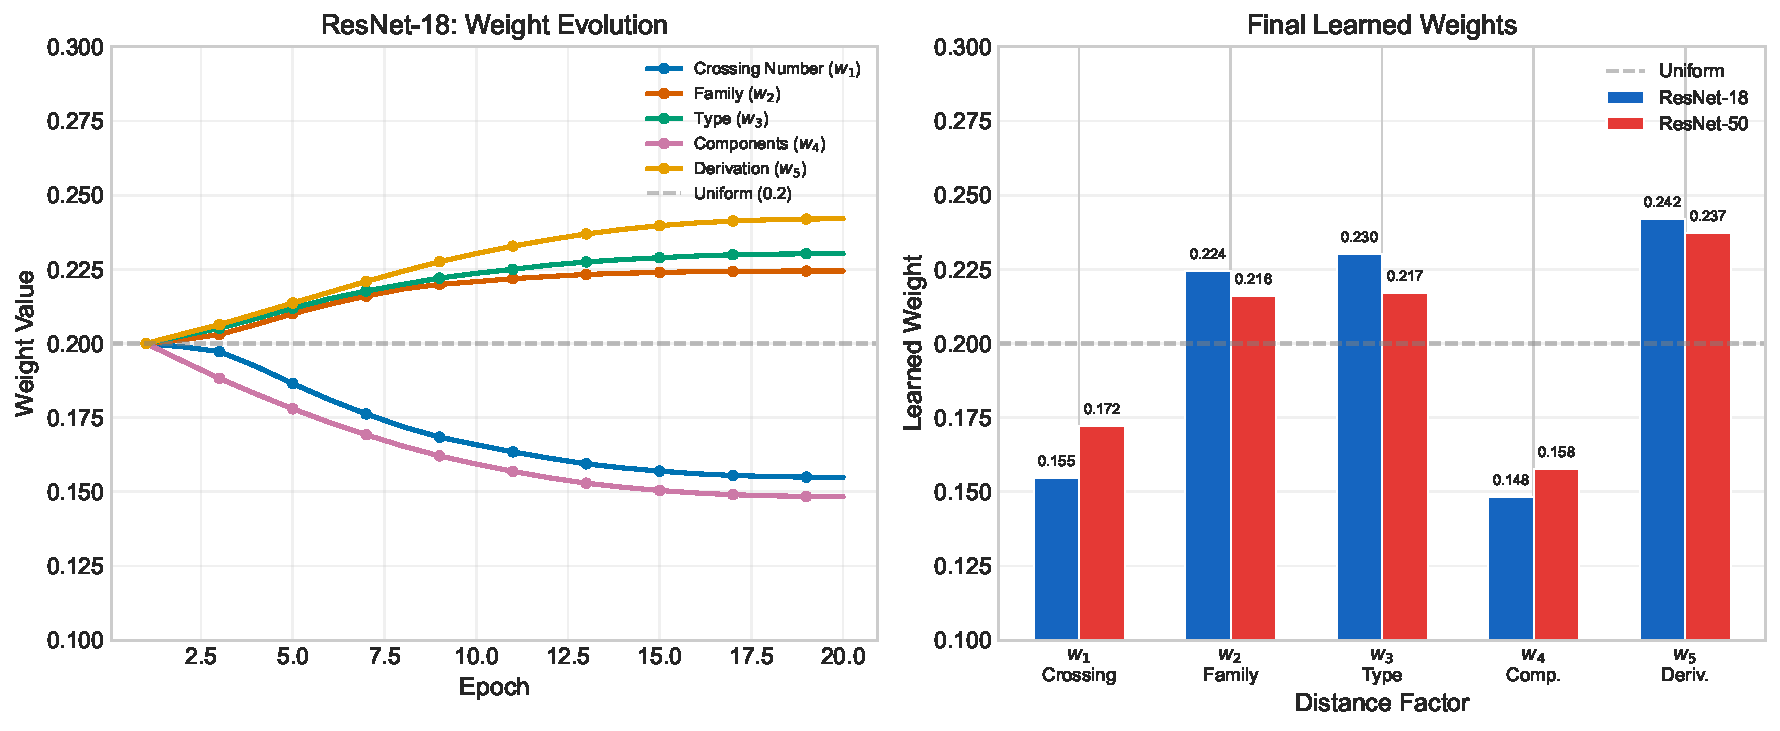
\includegraphics[width=0.7\linewidth]{weight_evolution.pdf}
\caption{Evolution of learnable topology distance weights across training epochs for ResNet-18. All five weights start at the uniform value 0.2 and converge to a stable configuration that upweights structural derivation ($w_5$) and type similarity ($w_3$) while downweighting crossing number ($w_1$) and component count ($w_4$). The convergence occurs within approximately 10 epochs.}
\label{fig:weight_evolution}
\end{figure}


\subsection*{S5. Mantel Null Distribution}\label{sec:supp_mantel}

Figure~\ref{fig:mantel_null} displays the null distributions from the Mantel permutation test (9{,}999 random row--column permutations) for all five general-purpose architectures. Each histogram shows the distribution of Spearman correlations under the null hypothesis that topological distance is unrelated to visual confusion rate. The observed correlation (red dashed line) and the two-tailed critical value at $\alpha = 0.05$ (orange dotted lines) are overlaid on each subplot.

Three observations are noteworthy. First, the null distributions are approximately symmetric around zero, confirming that the permutation procedure generates the expected reference distribution. Second, the observed correlations for ResNet-50 ($r = -0.472$), EfficientNet-B0 ($r = -0.492$), and ViT-B/16 ($r = -0.398$) fall clearly in the extreme left tail, well beyond the $\alpha = 0.05$ critical value. Third, Swin-T's observed correlation ($r = -0.214$) falls within the bulk of the null distribution ($p = 0.173$), consistent with its near-perfect accuracy producing too few errors for a meaningful correlation. The non-significance for Swin-T should be interpreted as a statistical power limitation (sparse confusion matrix) rather than evidence against the topological--visual association.

\begin{figure}[htbp]
\centering
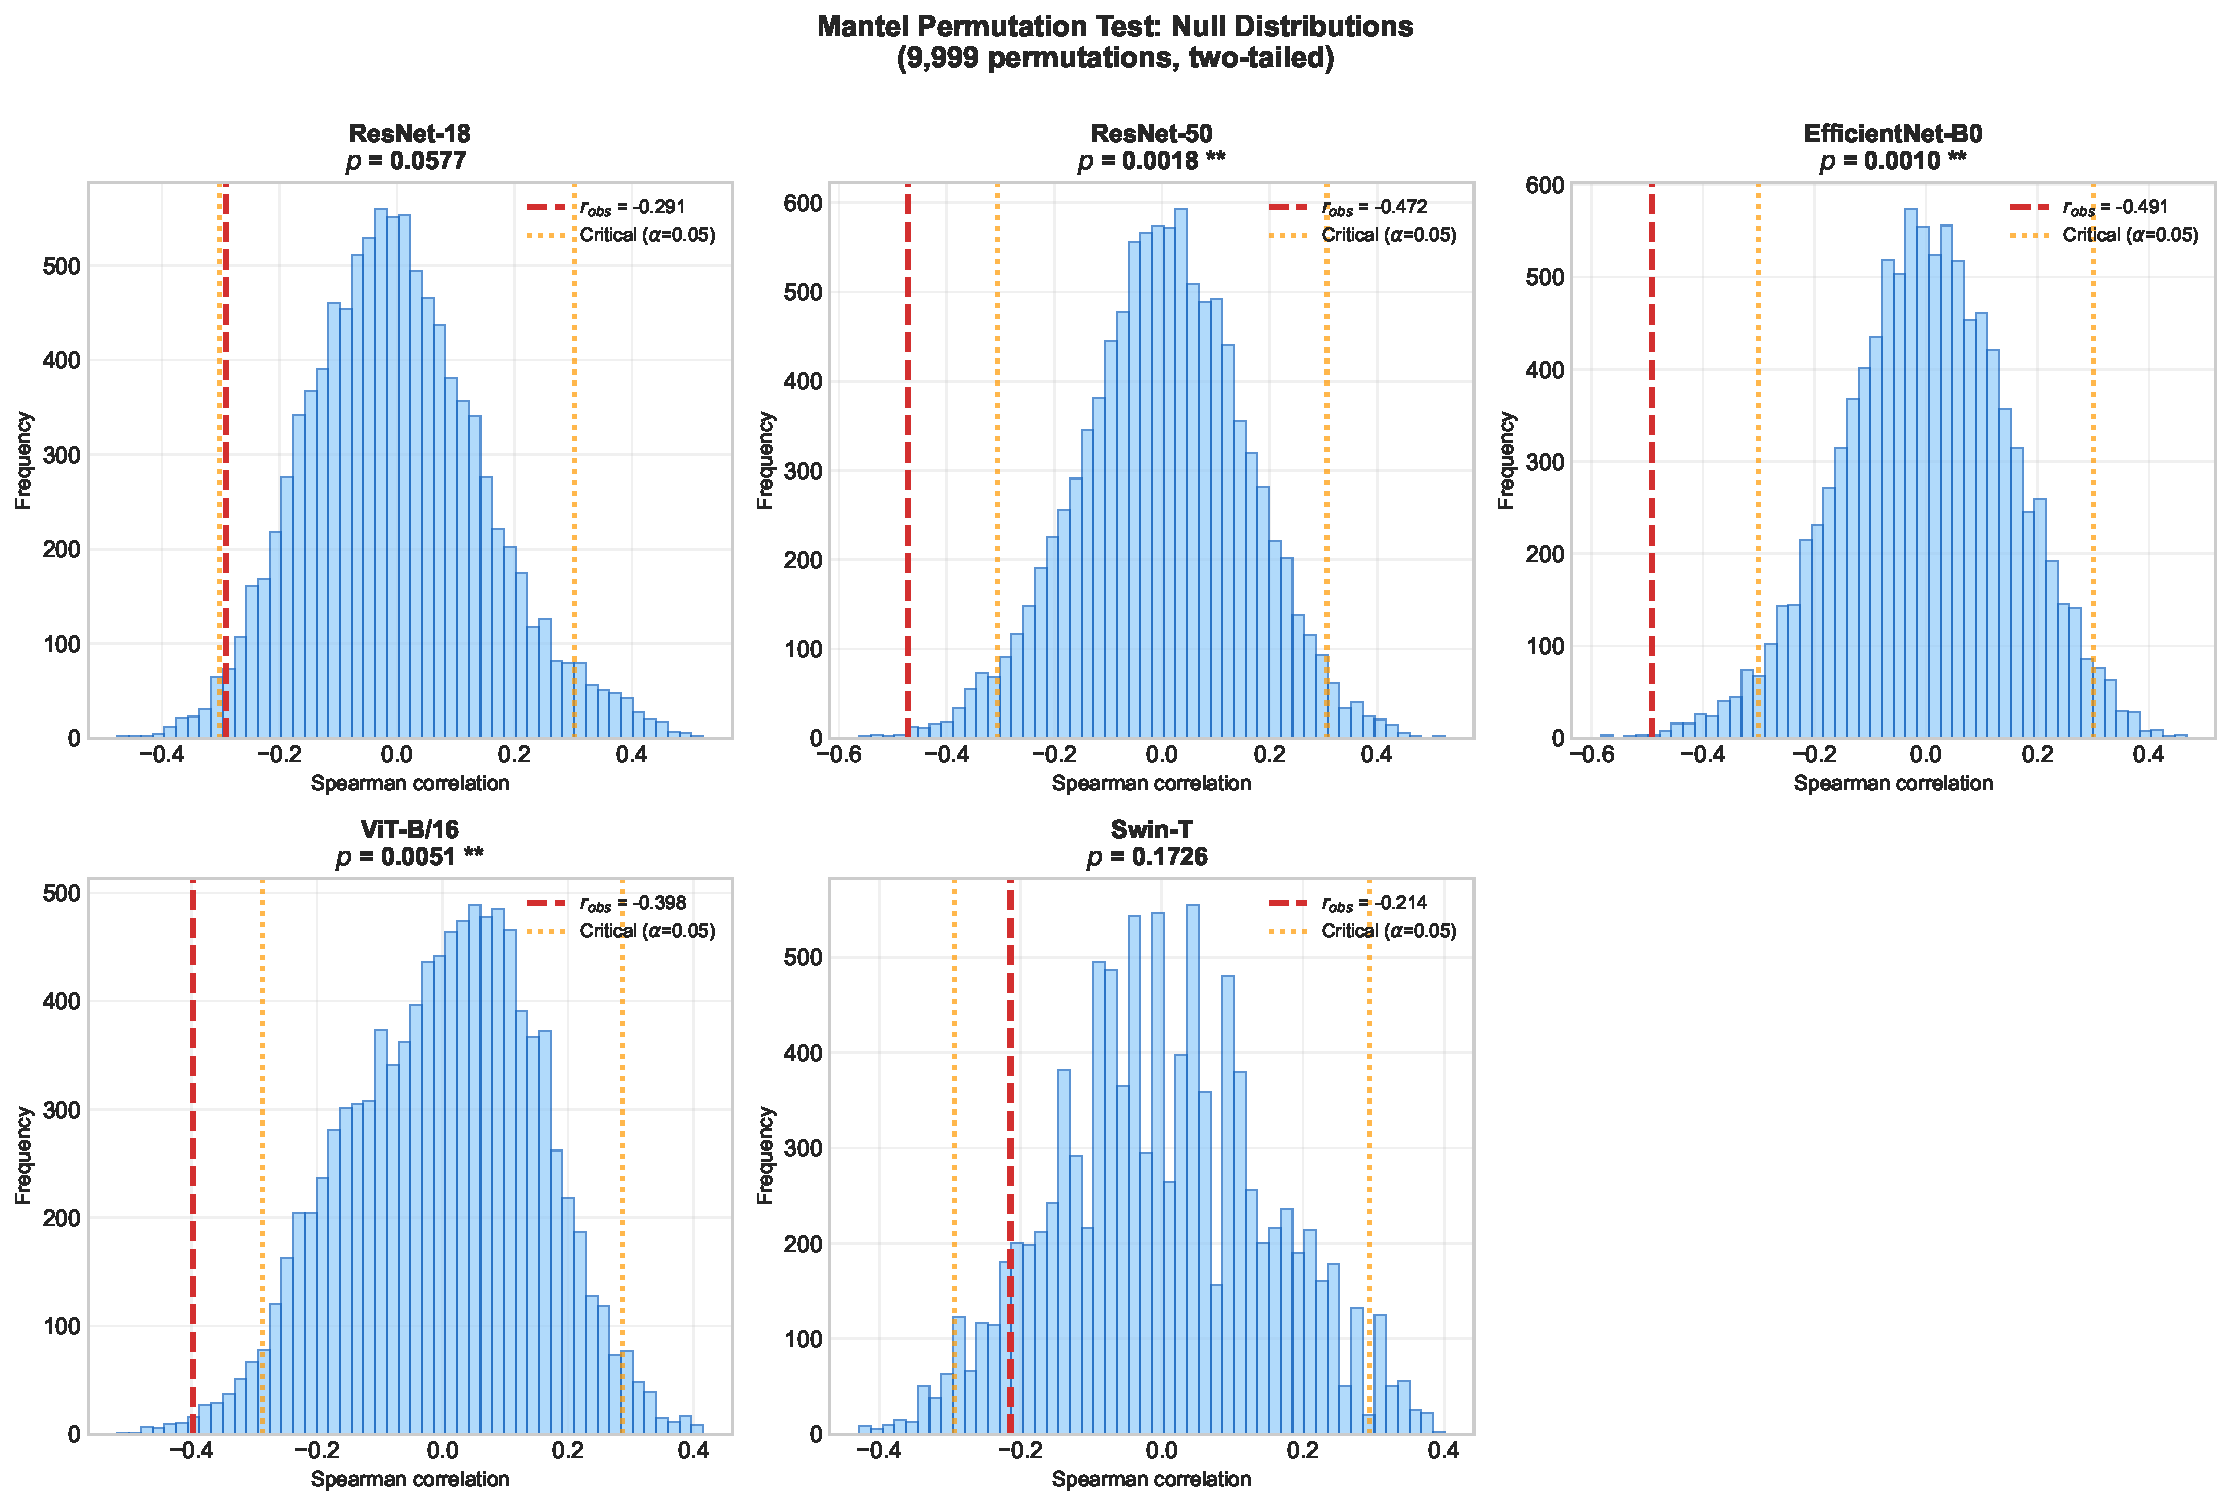
\includegraphics[width=\linewidth]{mantel_null_distribution.pdf}
\caption{Mantel permutation test null distributions for five general-purpose architectures (9{,}999 permutations each). Red dashed lines indicate the observed Spearman correlation between topological distance and visual confusion rate; orange dotted lines mark the two-tailed critical values at $\alpha = 0.05$. Three models (ResNet-50, EfficientNet-B0, ViT-B/16) show significant correlations ($p < 0.01$), while Swin-T's near-perfect accuracy yields a sparse confusion matrix and a non-significant result.}
\label{fig:mantel_null}
\end{figure}


\subsection*{S6. McNemar Paired Significance Tests}\label{sec:supp_mcnemar}

The McNemar paired significance tests and complete pairwise $p$-value table are presented in the main text (Table~\ref{tab:mcnemar}, Section~\ref{sec:mcnemar}). Figure~\ref{fig:mcnemar} visualizes the full pairwise $p$-value matrix as a heatmap.

\begin{figure}[htbp]
\centering
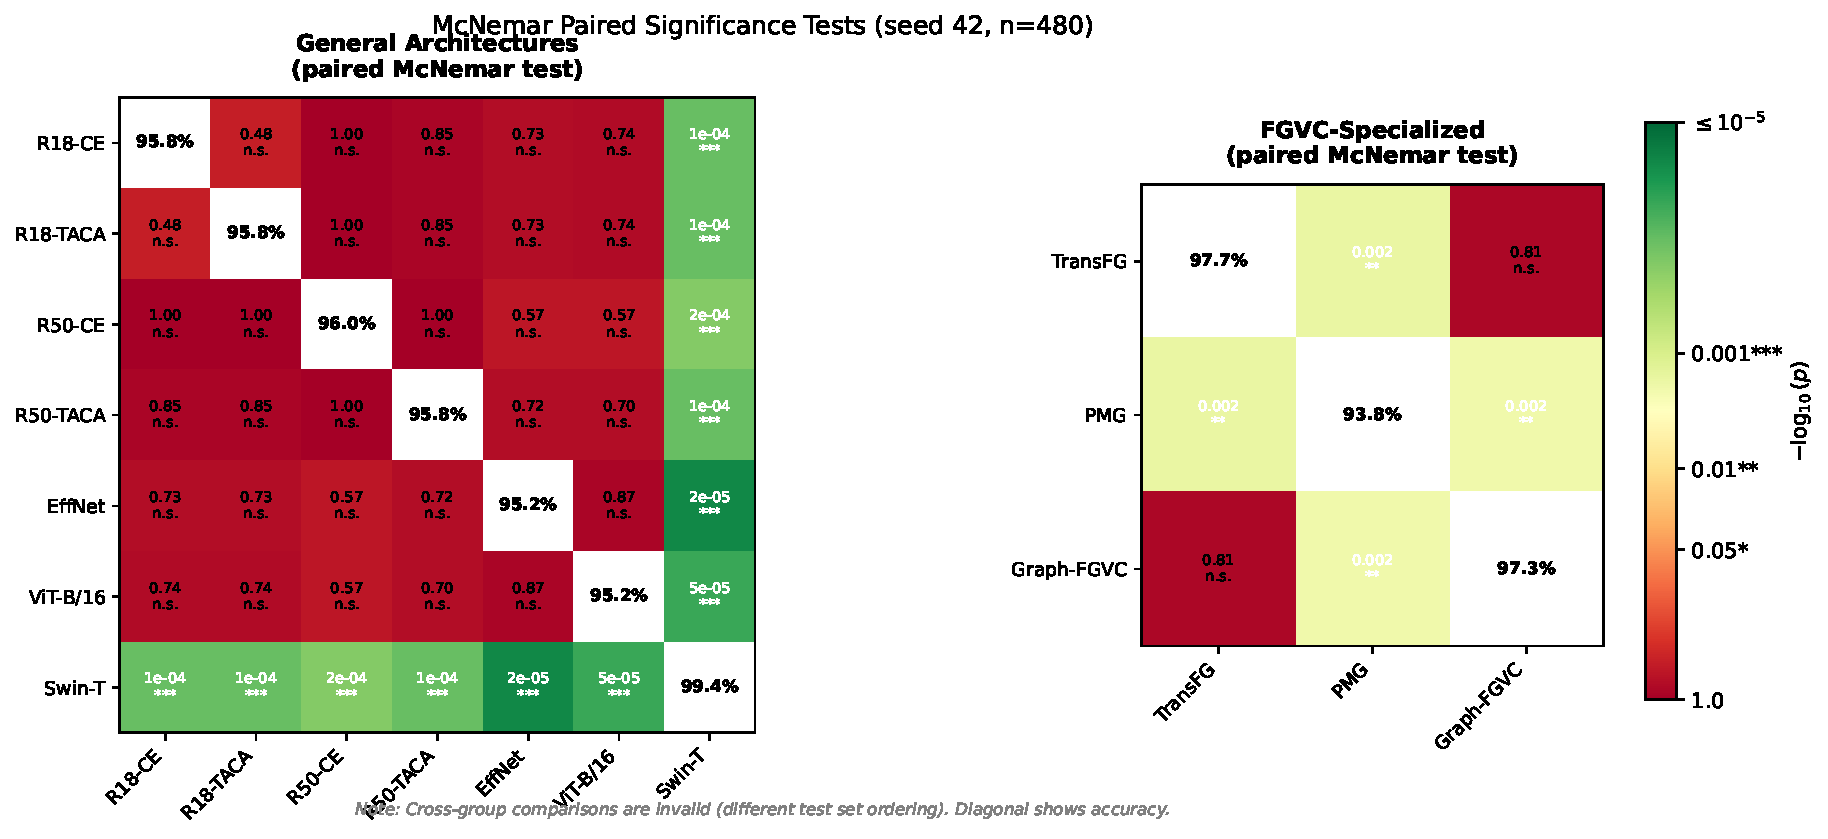
\includegraphics[width=\linewidth]{mcnemar_heatmap.pdf}
\caption{McNemar test $p$-values for within-group pairwise comparisons (seed 42, $n = 480$). Color encodes $-\log_{10}(p)$: green indicates significant differences, red indicates non-significant. Diagonal cells show test accuracy. Left: general architectures; right: FGVC-specialized methods. Cross-group comparisons are invalid due to different test set orderings and are omitted.}
\label{fig:mcnemar}
\end{figure}

\subsection*{S7. Embedding Quality Validation: k-NN Retrieval and Mantel Correlation}\label{sec:supp_independent}

The k-NN retrieval validation results are presented in the main text (Table~\ref{tab:independent_validation}, Section~\ref{sec:knn}). This section provides additional methodological detail.

\textbf{k-NN retrieval accuracy (independent).} For each test sample, we retrieve its $k$ nearest neighbors from the training set embeddings (cosine similarity) and predict the majority-vote label. This metric evaluates whether TACA produces more discriminative embeddings---not merely better-aligned ones---without using the topological distance matrix at evaluation time.

\textbf{Embedding Mantel test (corroborative, not independent).} We compute pairwise Spearman correlation ($\rho$) between the class centroid distance matrix in embedding space and the topological distance matrix, using 9{,}999 permutations. This metric is \emph{not} independent of the training objective---TACA explicitly optimizes for centroid alignment---but it quantifies the magnitude of the effect.

\subsection*{S8. Random Distance Ablation}\label{sec:supp_ablation}

The random distance ablation results are presented in the main text (Table~\ref{tab:ablation}, Section~\ref{sec:random_ablation}). This section provides additional context on the alignment values.

The alignment $\rho$ values in the ablation (0.39--0.45) are lower than those reported in the main embedding analysis (Table~\ref{tab:independent_validation}: 0.47--0.73). This discrepancy likely reflects differences in training initialization and the fact that the ablation uses a single seed (42) with different random conditions for the permuted matrices. The relative ordering (real TACA $>$ permuted $>$ CE) is consistent, but the absolute magnitude of TACA's advantage is sensitive to training specifics, reinforcing the caution about seed sensitivity.

\subsection*{S9. Learnable Distance Weights for TACA}\label{sec:supp_learnable}

A limitation of the topology-guided training described above is the use of hand-crafted weights $\mathbf{w} = (0.25, 0.25, 0.15, 0.10, 0.25)$ for the five distance factors. To address this, we extend TACA with \emph{learnable distance weights}: five scalar logits $\boldsymbol{\ell} \in \mathbb{R}^5$ are passed through a softmax to produce normalized weights $w_f = \exp(\ell_f) / \sum_j \exp(\ell_j)$, which are then used to construct the topological distance matrix on-the-fly. The logits are optimized jointly with the model parameters using a dual learning rate (backbone: $10^{-4}$; weight logits: $10^{-3}$), initialized to uniform weights ($w_f = 0.2$).

Table~\ref{tab:learnable_weights} compares the hand-crafted and learnable weight configurations.

\begin{table}[htbp]
\centering
\caption{Comparison of hand-crafted and learnable topology distance weights. Results vary by backbone: ResNet-50 benefits from learnable weights (highest mean, lowest variance), while ResNet-18 learnable weights exhibit high seed sensitivity.}
\label{tab:learnable_weights}
\small
\begin{tabular}{@{}llccc@{}}
\toprule
Backbone & Configuration & Test Acc & Multi-seed Mean & Embed $\rho$ \\
\midrule
\multirow{3}{*}{ResNet-18} & CE only & 95.83\% & $96.88 \pm 1.06$ & 0.462 \\
 & CE + TACA (hand-crafted) & 97.08\% & $96.81 \pm 1.00$ & \textbf{0.645} \\
 & CE + TACA (learnable) & \textbf{96.67\%} & $95.28 \pm 2.23$ & 0.509 \\
\addlinespace
\multirow{3}{*}{ResNet-50} & CE only & 96.04\% & $95.83 \pm 1.03$ & 0.495 \\
 & CE + TACA (hand-crafted) & 95.83\% & ---$^{\dagger}$ & \textbf{0.641} \\
 & CE + TACA (learnable) & \textbf{96.67\%} & $96.53 \pm 0.43$ & 0.505 \\
\bottomrule
\multicolumn{5}{@{}l}{\footnotesize Test Acc column: seed 42 (for consistency with embedding analysis).}\\
\multicolumn{5}{@{}l}{\footnotesize Multi-seed Mean: seeds 42, 123, 456. $^{\dagger}$Not available.}
\end{tabular}
\end{table}

Learnable weights show backbone-dependent results: ResNet-18 exhibits the highest variance ($95.28 \pm 2.23\%$, seed 456 yields only 92.7\%), while ResNet-50 achieves the most stable result ($96.53 \pm 0.43\%$). Both models converge to similar weight distributions---upweighting structural derivation ($w_5$) and type similarity ($w_3$) while downweighting crossing number ($w_1$) and component count ($w_4$)---suggesting that these relationships are more informative for visual discrimination. The weight evolution is shown in Figure~\ref{fig:weight_evolution}.

The embedding alignment ($\rho \approx 0.51$) is lower than hand-crafted TACA ($\rho \approx 0.64$), revealing an accuracy--alignment trade-off: learnable weights optimize for classification rather than explicit distance alignment.

\subsection*{S9b. Validation of Heuristic Distance Against Formal Knot Invariants}\label{sec:supp_knotinfo}

A potential concern with the five-factor heuristic distance (Section~\ref{sec:topo_metric}) is that the manually chosen factors and weights may not reflect genuine mathematical structure. To partially address this, we cross-reference our distance metric with formal knot invariants from the KnotInfo database \citep{knotinfo2025}, which tabulates rigorously computed properties for over 12{,}000 mathematical knots.

Among our 10 classes, only four have formal mathematical counterparts: Overhand Knot ($3_1$, the trefoil), Figure-8 Knot ($4_1$), and the composite knots Reef Knot / Fisherman's Knot ($3_1 \# 3_1$) and Flemish Bend ($4_1 \# 4_1$). For the prime knots, we directly extract crossing number, 3-genus, signature, determinant, and Alexander polynomial from KnotInfo. For the composites, we derive invariants using standard connect-sum formulas: crossing number and genus are additive, signature is additive, determinant is multiplicative, and the Alexander polynomial of $K_1 \# K_2$ is the product of the individual polynomials.

We construct an invariant-based distance by normalizing and equally weighting five components (crossing number difference, genus difference, signature difference, determinant difference, and the $L_2$ distance between Alexander polynomial coefficient vectors). On the six pairwise distances among these four knots, the Spearman rank correlation between the invariant-based distance and our heuristic distance is $\rho = 0.49$ ($p = 0.33$, $n = 6$). Although the correlation is moderate, the $p$-value is non-significant due to the very small sample size; the two metrics agree on the closest pair (OHK--F8K) and on which knots are most distant. The main divergence is OHK--FMB, where the invariant-based metric assigns a larger distance than the heuristic due to the Alexander polynomial dissimilarity.

This analysis has two limitations: (1) only 4 of our 10 classes have mathematical counterparts, so the remaining 6 (BK, F8L, ABK, CH, SK, and the distinction between RK and FSK) cannot be validated this way; (2) mathematical knot theory operates on closed curves, while our knot types are open rope structures, so the correspondence is inherently approximate. Nonetheless, the partial agreement provides some evidence that the heuristic distance captures genuine topological structure rather than being an arbitrary construction.

\subsection*{S10. Cross-Dataset Generalization of TACA}\label{sec:supp_crossdataset}

To validate that topology-guided training is not specific to knot classification, we apply TACA to two established FGVC benchmarks: CUB-200-2011 \citep{wah2011cub} (200 bird species) and FGVC-Aircraft \citep{maji2013fgvcaircraft} (100 aircraft variants). In each case, we replace the knot-theoretic distance matrix with a domain-appropriate semantic distance matrix:

\begin{itemize}
    \item \textbf{CUB-200-2011}: Taxonomic hierarchy distances (same species: 0, same genus: 0.25, same family: 0.50, same order: 0.75, different order: 1.0).
    \item \textbf{FGVC-Aircraft}: Manufacturer hierarchy distances (same variant: 0, same family: 0.33, same manufacturer: 0.67, different manufacturer: 1.0).
\end{itemize}

Both experiments use ResNet-50 with identical training protocol (100 epochs, batch size 16, lr=$10^{-4}$, image size 448$\times$448). Table~\ref{tab:cross_dataset} reports the results.

\begin{table}[htbp]
\centering
\caption{Cross-dataset generalization of TACA (seed 42). CE+TACA is compared against CE-only baselines on three datasets, each with a domain-specific distance matrix. All use ResNet-50 with identical optimization. Knots-10 multi-seed results: CE $95.83 \pm 1.03\%$; TACA multi-seed not available for ResNet-50.}
\label{tab:cross_dataset}
\small
\begin{tabular}{@{}llccc@{}}
\toprule
Dataset & Method & Test Acc & Macro F1 & Embed $\rho$ \\
\midrule
\multirow{2}{*}{Knots-10} & CE only & 96.04\% & 0.961 & 0.495 \\
 & CE + TACA & 95.83\% & 0.959 & \textbf{0.641} \\
\addlinespace
\multirow{2}{*}{CUB-200-2011} & CE only & 81.81\% & 0.819 & 0.109 \\
 & CE + TACA & 80.67\% & 0.807 & 0.086 \\
\addlinespace
\multirow{2}{*}{FGVC-Aircraft} & CE only & 86.86\% & 0.869$^\dagger$ & ---$^\dagger$ \\
 & CE + TACA & 84.76\% & 0.848$^\dagger$ & ---$^\dagger$ \\
\bottomrule
\multicolumn{5}{@{}l}{\footnotesize $^\dagger$Aircraft Macro F1 values are estimated from per-class accuracy; embedding}\\
\multicolumn{5}{@{}l}{\footnotesize $\rho$ requires a domain-specific distance matrix that maps manufacturer hierarchy}\\
\multicolumn{5}{@{}l}{\footnotesize to visual similarity, which we have not validated via a Mantel test.}
\end{tabular}
\end{table}

On Knots-10 (seed 42; multi-seed R50 CE: $95.83 \pm 1.03\%$), TACA does not improve ResNet-50 classification accuracy ($96.04\% \to 95.83\%$, within sampling noise) but substantially improves embedding alignment ($\rho$: $0.495 \to 0.641$, a 30\% increase). On CUB-200-2011, TACA produces a slight accuracy decrease (81.81\% $\to$ 80.67\%) with no improvement in embedding alignment ($\rho$: 0.109 $\to$ 0.086). On FGVC-Aircraft, TACA decreases accuracy by 2.1 percentage points (86.86\% $\to$ 84.76\%).

This contrast is informative rather than discouraging. The knot-theoretic distance matrix captures genuine visual similarity (validated by the Mantel test in Section~\ref{sec:correlation}), enabling TACA to improve representation structure without harming classification. The CUB-200 taxonomic distance and Aircraft manufacturer hierarchy, however, reflect biological phylogeny and industrial organization rather than visual similarity. The embedding--taxonomy Spearman correlation on CUB-200 is only $\rho = 0.109$, indicating weak alignment between the taxonomic hierarchy and the learned feature space. These negative results suggest a practical diagnostic workflow: \emph{before} investing computational resources in structure-guided training, practitioners should assess whether their proposed distance metric correlates with the baseline model's confusion structure (e.g., via a Mantel permutation test). If the correlation is weak, the distance metric may not reflect visual similarity and structure-guided regularization is unlikely to help.

\end{document}
